\chapter{Coordinate Systems on the Celestial Sphere}
\label{ch:coords}

Every direction in the sky is a point on the celestial sphere of Section~\ref{sec:celestial_sphere_primer}. Two angles fix such a point, in the same way that latitude and longitude fix a town on the Earth. The two angles depend on a choice of pole and of a zero point on the equator around that pole. An observer on the ground uses the zenith as the pole. A star catalogue uses the celestial pole. The planets move most simply about the pole of the Earth's orbit, and the Milky Way is simplest about the pole of its own disk.

All four systems describe the same direction. Going from one to another is a turn of the axes, written as a matrix acting on a unit vector. Two physical effects then move a star away from where the geometry puts it. The air bends its light, and the motion of the Earth tilts it.

% ==============================================================================
\section{The Equatorial Coordinate System}
\label{co:sec:equatorial}

Chapter~\ref{ch:time} introduced the celestial poles, the celestial equator and the vernal equinox $\hat\gamma$, and built a sidereal clock from them (Section~\ref{sec:celestial_sphere_primer}, Eq.~\eqref{eq:lst_def}).

Words like ``north of the equator'' or ``east of the equinox'' cannot yet be computed with. To find the angle between two stars, or to turn to another frame, a direction has to be a vector.

Think of a town on a globe. Its latitude says how far north of the equator it lies. Its longitude says how far east of Greenwich it lies, counted along the equator. An arrow from the centre of the globe to the town is fixed by these two angles. Its height above the plane of the equator is the sine of the latitude. Its shadow on that plane has the cosine of the latitude as its length, and it points in the direction given by the longitude.

The sky uses the same two angles. Declination plays the part of latitude, and right ascension plays the part of longitude, with $\hat\gamma$ in place of Greenwich. A direction on the sky is a unit vector whose three components are products of sines and cosines of these two angles.

Vega is at right ascension $18^{\rm h}36^{\rm m}56^{\rm s}=279.23^\circ$ and declination $+38.78^\circ$. Its arrow rises $\sin38.78^\circ=0.626$ above the plane of the equator. Its shadow has length $\cos38.78^\circ=0.779$ and points $279.23^\circ$ round from $\hat\gamma$. The two components in the plane are $0.779\cos279.23^\circ=0.125$ and $0.779\sin279.23^\circ=-0.769$.

The picture is an arrow from the centre of a ball to a dot on its surface, with the arrow's shadow on the equatorial plane.

The same construction is the spherical polar coordinates of mechanics, with polar angle $90^\circ-\delta$. It gave the line of sight to a binary in Chapter~\ref{ch:twobody} (Section~\ref{sec:coord_orbital_elements}), and it gives the local directions on the sky used for proper motions in Chapter~\ref{ch:astrometry}. It is pure geometry, so none of the six principles enters. What it gives is the unit vector on which every later formula acts.

\paragraph{The two angles.} The \textbf{declination} $\delta\in[-90^\circ,+90^\circ]$ is the angle of a direction north ($+$) or south ($-$) of the celestial equator. The great circle through the two poles and a star is the star's \textbf{hour circle}. The \textbf{right ascension} $\alpha$ is the angle along the celestial equator from $\hat\gamma$ eastward to the hour circle. It runs from $0^{\rm h}$ to $24^{\rm h}$, with $1^{\rm h}=15^\circ$ (Eq.~\eqref{eq:time_angle_conversion}). Both are shown in Figure~\ref{fig:declination}.

\paragraph{The unit vector.} Put the $z$ axis toward the north celestial pole and the $x$ axis toward $\hat\gamma$. The $y$ axis then points to $\alpha=6^{\rm h}$, which makes the three axes right-handed. Split the direction $\hat{\mathbf r}$ of a star into a part along the pole and a part in the plane of the equator,
\begin{align}
	\hat{\mathbf r}
	&\eqby{1} \sin\delta\,\hat{\mathbf z}+\cos\delta\,\big(\cos\alpha\,\hat{\mathbf x}+\sin\alpha\,\hat{\mathbf y}\big) \nonumber\\
	&\eqby{2} \cos\delta\cos\alpha\,\hat{\mathbf x}+\cos\delta\sin\alpha\,\hat{\mathbf y}+\sin\delta\,\hat{\mathbf z}.
\end{align}
\begin{explain}
	\item The angle between $\hat{\mathbf r}$ and the plane of the equator is $\delta$. So the part along the pole is $\sin\delta$, and the shadow in the plane has length $\cos\delta$ and makes the angle $\alpha$ with $\hat{\mathbf x}$.
	\item Multiplying out the bracket.
\end{explain}
We write the three components as a column, labelled by the frame they belong to,
\begin{equation}
	\boxed{\hat{\mathbf r}_{\rm eq}=\begin{pmatrix}\cos\delta\cos\alpha\\ \cos\delta\sin\alpha\\ \sin\delta\end{pmatrix}.}
	\label{eq:unit_vector_eq}
\end{equation}
Its length is one for every $(\alpha,\delta)$. It does not depend on the time or on where on the Earth the observer stands, because the grid turns with the stars.

\begin{figure}[htbp]
	\centering
	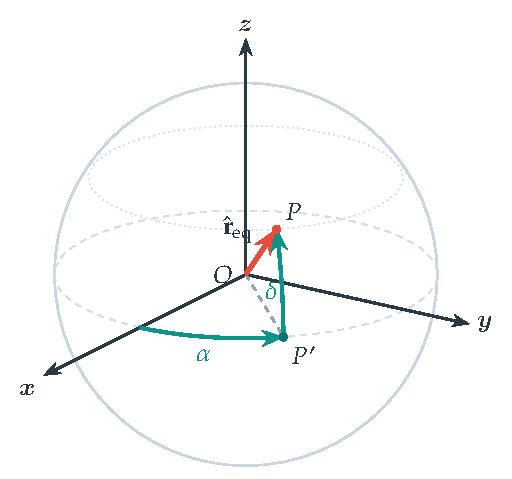
\includegraphics{fig_ch2_prob_equatorial_unit_vector.pdf}
	\caption{The unit vector $\hat{\mathbf r}_{\rm eq}$ toward a point $P$ in the equatorial frame, with its right ascension $\alpha$ measured from the $x$ axis and its declination $\delta$ measured up from the equatorial plane.}
	\label{co:fig:unit_vector}
\end{figure}

The values of $(\alpha,\delta)$ in a catalogue change only slowly, through the star's own motion across the sky and through precession. The daily rising and setting of the stars comes from the observer's horizon turning under this fixed grid.

\begin{figure}[htbp]
	\centering
	\begin{minipage}[t]{0.48\textwidth}
		\centering
		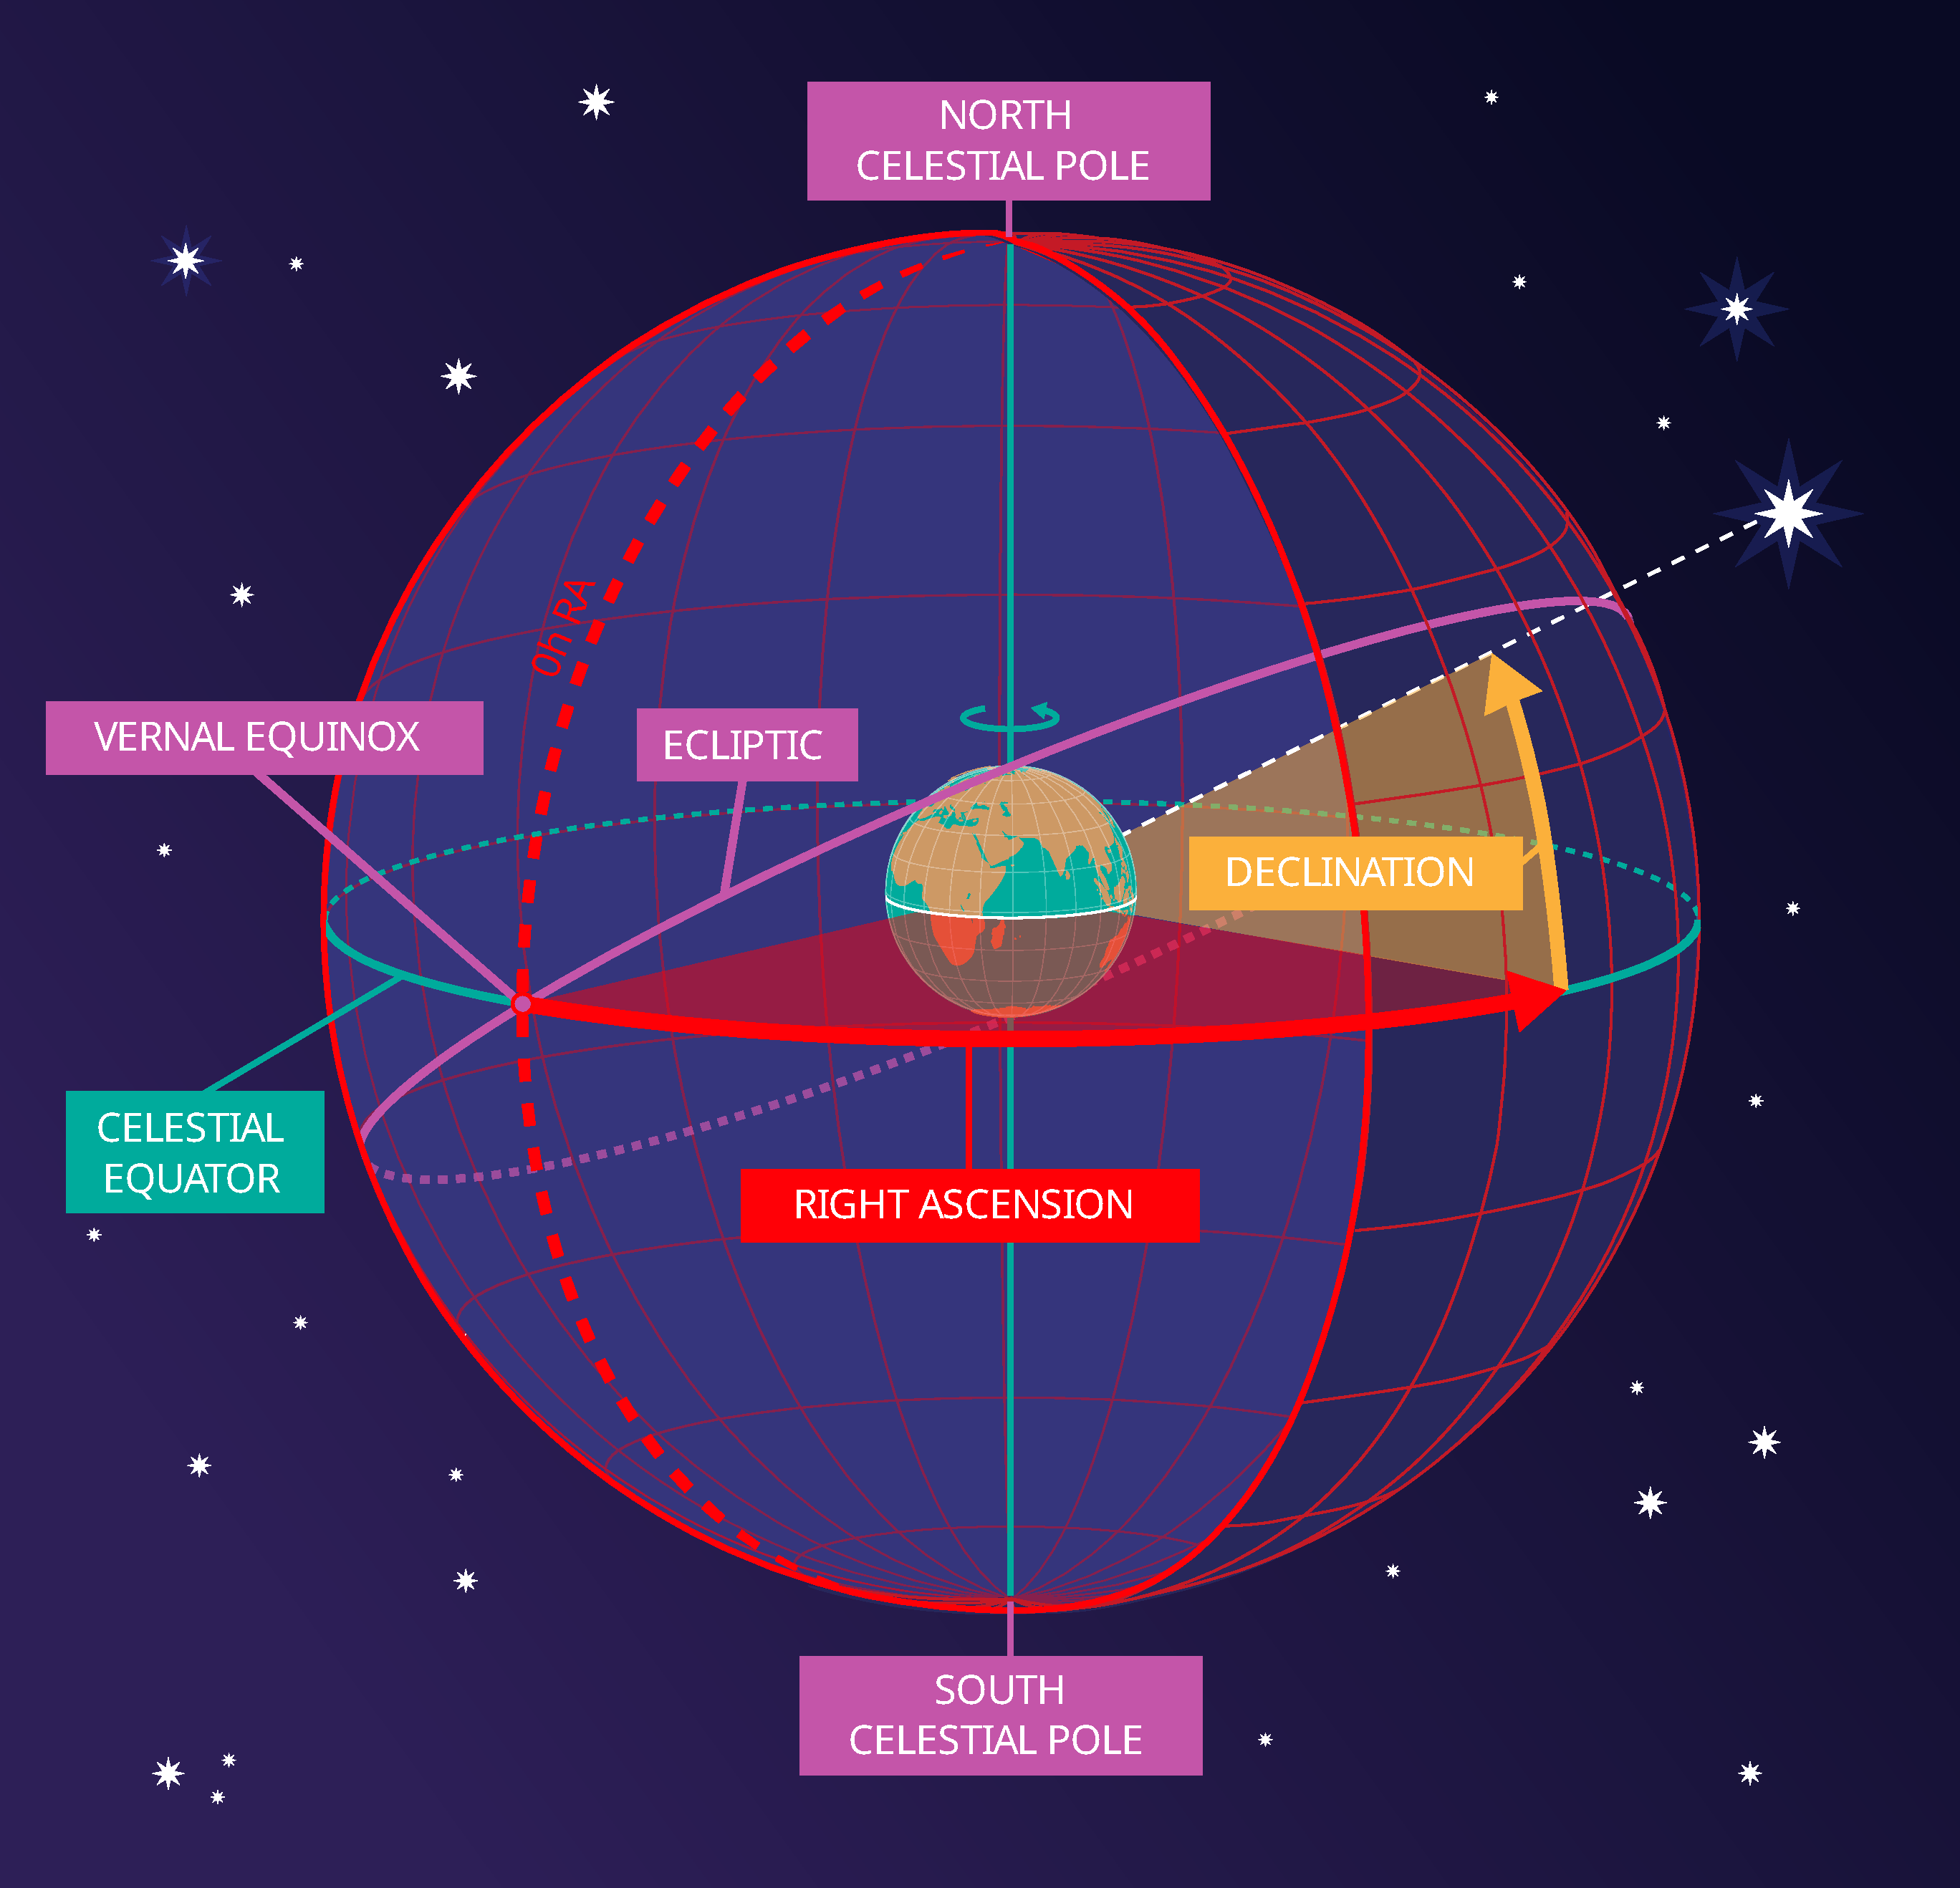
\includegraphics[width=\linewidth]{declination_celestial_coordinates_en_bviPcZn.pdf}
		\caption{The celestial sphere around the Earth, with the north and south celestial poles, the celestial equator, the ecliptic, the vernal equinox, and the right ascension and declination of a star.}
		\label{fig:declination}
		\label{fig:ch2_prob_declination}
	\end{minipage}
	\hfill
	\begin{minipage}[t]{0.48\textwidth}
		\centering
		\resizebox{\linewidth}{!}{%
		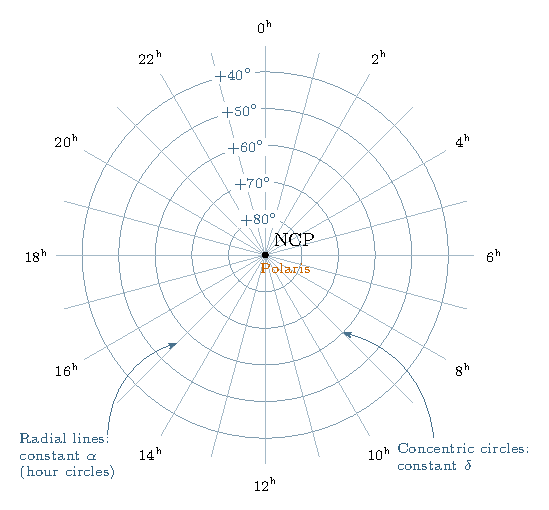
\includegraphics{fig_ch2_ra_dec_polar_grid.pdf}%
		}
		\caption{The equatorial grid near the north celestial pole, as seen by an observer facing north. Radial lines are hour circles $1^{\rm h}$ apart. Circles are parallels of constant $\delta$, $10^\circ$ apart.}
		\label{fig:ra_dec_polar_grid}
	\end{minipage}
\end{figure}

The grid of Figure~\ref{fig:ra_dec_polar_grid} is the one that planetarium software draws on the real sky (Figure~\ref{fig:ra_dec_real_photo}). In both, $\alpha$ grows clockwise around the pole for an observer facing north. The reason is that a star of larger $\alpha$ reaches the meridian later, so at any moment it lies further east, and east is on the right for someone facing north.

\begin{figure}[htbp]
	\centering
	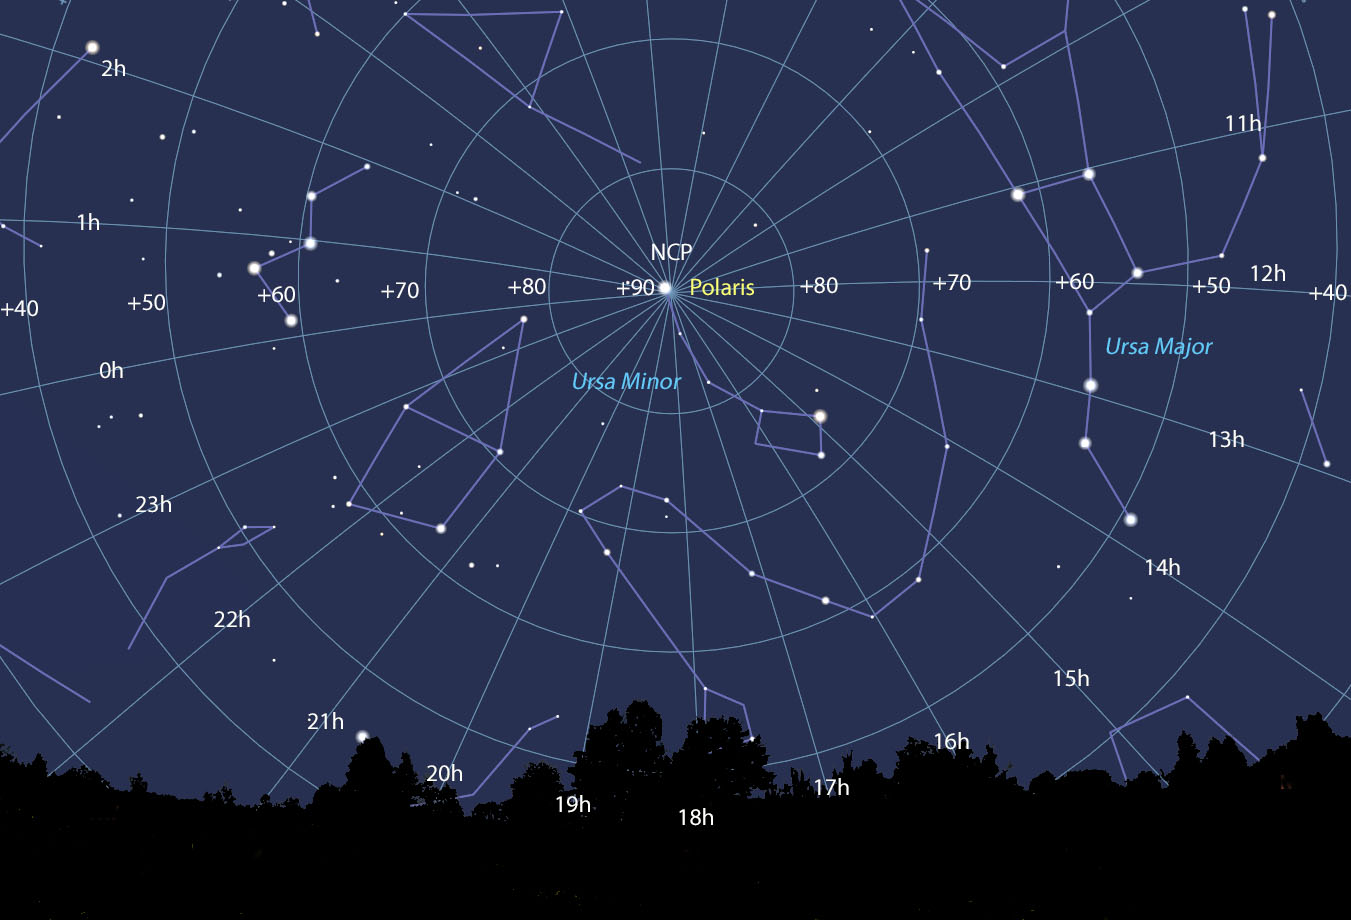
\includegraphics[width=0.6\linewidth]{RA-Dec-celestial-pole.jpg}
	\caption{An equatorial grid drawn over the sky near the north celestial pole, with Polaris and the constellations Ursa Minor and Ursa Major.}
	\label{fig:ra_dec_real_photo}
\end{figure}

The local sidereal time and the hour angle of Chapter~\ref{ch:time} are two more angles on the same sphere. Figure~\ref{fig:lst_meridian_schematic} marks $\hat\gamma$, the observer's meridian and a star $S$ together. The right ascension now on the meridian is the local sidereal time, Eq.~\eqref{eq:lst_def}. In that figure the star is still east of the meridian. As the Earth turns, the LST grows while the star's $\alpha$ stays fixed. Figure~\ref{fig:lst_meridian_schematic_later} shows the same sky later, after the meridian has passed the star. The arc from the meridian back to the star is then the hour angle $H$, defined in Section~\ref{co:sec:horizontal}. In the earlier figure the same arc points the other way and has length $-H$.

\begin{figure}[htbp]
	\centering
	\begin{minipage}[t]{0.48\textwidth}
		\centering
		\resizebox{\linewidth}{!}{%
		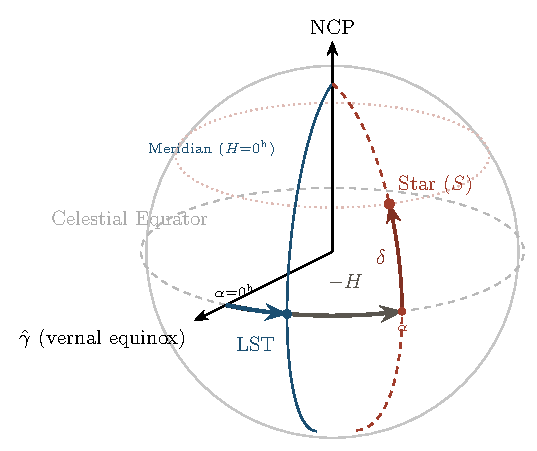
\includegraphics{fig_ch2_lst_meridian_schematic.pdf}%
		}
		\caption{The vernal equinox $\hat\gamma$, the observer's meridian and a star $S$ at $(\alpha,\delta)$ east of the meridian, on one celestial sphere.}
		\label{fig:lst_meridian_schematic}
	\end{minipage}
	\hfill
	\begin{minipage}[t]{0.48\textwidth}
		\centering
		\resizebox{\linewidth}{!}{%
		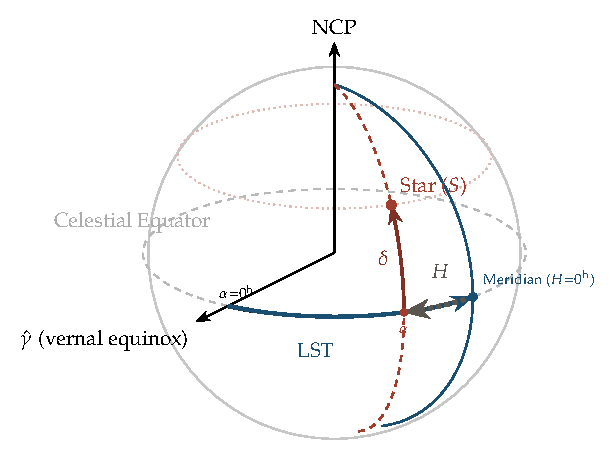
\includegraphics{fig_ch2_lst_meridian_schematic_later.pdf}%
		}
		\caption{The same sky as Figure~\ref{fig:lst_meridian_schematic} at a later instant. $\hat\gamma$ and $S$ are unchanged, and the meridian has moved past the star.}
		\label{fig:lst_meridian_schematic_later}
	\end{minipage}
\end{figure}

\subsection{Coordinate Epochs}
\label{sec:coordinate_epochs}

The equinox $\hat\gamma$ that anchors the grid moves. The Earth's axis precesses, and $\hat\gamma$ slides west along the ecliptic by about $50.3''$ per year, Eq.~\eqref{eq:precession_rate}. A position $(\alpha,\delta)$ therefore means nothing until it states the instant at which the grid was taken. That instant is the \textbf{epoch}. The standard today is J2000.0, and older catalogues used B1950.0. Some names carry the epoch. The pulsar PSR~J1939+2134 is named after its J2000 position, $\alpha\approx19^{\rm h}39^{\rm m}$ and $\delta\approx+21^\circ34'$.

Moving a position from one epoch to another needs two corrections. One is the precession of the grid, Eqs.~\eqref{eq:precess_alpha}--\eqref{eq:precess_delta}. The other is the star's own motion across the sky, its proper motion $(\mu_\alpha^*,\mu_\delta)$ of Chapter~\ref{ch:astrometry}. The two are independent, and over a few decades they simply add. To restate a catalogue from B1950.0 to J2000.0 with the stars held fixed, only the precession is needed.

% ==============================================================================
\section{Turning the Axes}
\label{co:sec:rotation}

The equatorial frame gives each star a column of three numbers, Eq.~\eqref{eq:unit_vector_eq}.

The other frames of the sky put their pole or their zero point somewhere else. We need the same star's components in those frames.

Think of a plan of a room drawn with the $x$ axis along one wall. A lamp stands $3\,\mathrm m$ along that wall from the corner. A friend draws the same room with axes turned $30^\circ$ anticlockwise. The lamp has not moved. Only the axes have. Its new coordinates are its distances measured along the friend's axes, and each of those is a dot product of the lamp's position with one of the friend's axes.

A star's direction does not change when we change frame either. The idea is that the new components are dot products with the new axes, so the matrix of the change has the new axes as its rows.

The lamp in numbers. The friend's axes are $(\cos30^\circ,\sin30^\circ)$ and $(-\sin30^\circ,\cos30^\circ)$ in the old frame. The lamp at $(3,0)$ has new coordinates $3\cos30^\circ=2.60$ and $-3\sin30^\circ=-1.50$. Stacking the two axes as rows gives the same answer as one matrix product,
\[
\begin{pmatrix}\cos30^\circ&\sin30^\circ\\-\sin30^\circ&\cos30^\circ\end{pmatrix}\begin{pmatrix}3\\0\end{pmatrix}=\begin{pmatrix}2.60\\-1.50\end{pmatrix}.
\]

The picture is two sets of axes with one origin, one turned against the other, and a single fixed arrow.

The same matrix is the passive rotation of mechanics and the change of basis of quantum mechanics. Chapter~\ref{ch:twobody} used two such turns to place an orbit in space, Eq.~\eqref{eq:orbital_frame_rotation}. It gives the two turns every frame of the sky is built from, and the fact that undoing a turn costs only a transpose.

\paragraph{The rule.} Let a new frame have orthonormal axes $\hat{\mathbf x}',\hat{\mathbf y}',\hat{\mathbf z}'$, each written by its components in the old frame. The new components of the direction $\hat{\mathbf r}$ are
\begin{align}
	\begin{pmatrix}x'\\y'\\z'\end{pmatrix}
	&\eqby{1} \begin{pmatrix}\hat{\mathbf x}'\cdot\hat{\mathbf r}\\ \hat{\mathbf y}'\cdot\hat{\mathbf r}\\ \hat{\mathbf z}'\cdot\hat{\mathbf r}\end{pmatrix}
	\eqby{2} \underbrace{\begin{pmatrix}\text{---}\ \hat{\mathbf x}'^{T}\ \text{---}\\ \text{---}\ \hat{\mathbf y}'^{T}\ \text{---}\\ \text{---}\ \hat{\mathbf z}'^{T}\ \text{---}\end{pmatrix}}_{\mathbf M}\begin{pmatrix}x\\y\\z\end{pmatrix}.
	\label{co:eq:rows_rule}
\end{align}
\begin{explain}
	\item In an orthonormal frame each component of a vector is its dot product with one axis.
	\item Each dot product is the row of the new axis's old components times the column of old components.
\end{explain}
The entries of $\mathbf M\mathbf M^{T}$ are the dot products of the new axes with each other,
\begin{equation}
	\mathbf M\mathbf M^{T}=\begin{pmatrix}\hat{\mathbf x}'\cdot\hat{\mathbf x}'&\hat{\mathbf x}'\cdot\hat{\mathbf y}'&\hat{\mathbf x}'\cdot\hat{\mathbf z}'\\ \hat{\mathbf y}'\cdot\hat{\mathbf x}'&\hat{\mathbf y}'\cdot\hat{\mathbf y}'&\hat{\mathbf y}'\cdot\hat{\mathbf z}'\\ \hat{\mathbf z}'\cdot\hat{\mathbf x}'&\hat{\mathbf z}'\cdot\hat{\mathbf y}'&\hat{\mathbf z}'\cdot\hat{\mathbf z}'\end{pmatrix}=\Id ,
	\qquad\text{so}\qquad
	\boxed{\mathbf M^{-1}=\mathbf M^{T}.}
	\label{co:eq:orthogonal}
\end{equation}
Going back to the old frame multiplies by the transpose, whose columns are the new axes. The determinant of $\mathbf M$ is $+1$ when the new axes are right-handed, and then $\mathbf M$ is a rotation. It is $-1$ when they are left-handed. The horizontal frame of Section~\ref{co:sec:horizontal} is such a case.

\paragraph{Turning about the $z$ axis.} Turn the $x$ and $y$ axes by $\theta$ about $z$, anticlockwise as seen from $+z$. The new axes are $\hat{\mathbf x}'=\cos\theta\,\hat{\mathbf x}+\sin\theta\,\hat{\mathbf y}$, $\hat{\mathbf y}'=-\sin\theta\,\hat{\mathbf x}+\cos\theta\,\hat{\mathbf y}$ and $\hat{\mathbf z}'=\hat{\mathbf z}$. Stacked as rows by Eq.~\eqref{co:eq:rows_rule},
\begin{equation}
	\begin{pmatrix} x' \\ y' \\ z' \end{pmatrix} = \underbrace{\begin{pmatrix} \cos\theta & \sin\theta & 0 \\ -\sin\theta & \cos\theta & 0 \\ 0 & 0 & 1 \end{pmatrix}}_{\mathbf R_z(\theta)}\begin{pmatrix} x \\ y \\ z \end{pmatrix}.
	\label{eq:z_axis_rotation_matrix}
\end{equation}

\paragraph{The same matrix from polar angles.} A second route uses angles in the plane of the turn. Take the turn about the $x$ axis, in the $y$--$z$ plane (Figure~\ref{co:fig:axes_rotation}). A point at distance $r$ from the axis and at angle $\Theta$ from the old $y$ axis has $(y,z)=(r\cos\Theta,r\sin\Theta)$. Measured from the new $y'$ axis, turned by $\theta$, its angle is $\Theta-\theta$. So
\begin{align}
	y'&=r\cos(\Theta-\theta)\eqby{1} r\cos\Theta\cos\theta+r\sin\Theta\sin\theta\eqby{2} y\cos\theta+z\sin\theta, \nonumber\\
	z'&=r\sin(\Theta-\theta)\eqby{1} r\sin\Theta\cos\theta-r\cos\Theta\sin\theta\eqby{2} -y\sin\theta+z\cos\theta .
\end{align}
\begin{explain}
	\item The angle-difference identities.
	\item $r\cos\Theta=y$ and $r\sin\Theta=z$.
\end{explain}
With $x'=x$ this is
\begin{equation}
	\mathbf R_x(\theta)=\begin{pmatrix}1&0&0\\0&\cos\theta&\sin\theta\\0&-\sin\theta&\cos\theta\end{pmatrix},
	\label{co:eq:Rx}
\end{equation}
which is $\mathbf R_z(\theta)$ with the axes relabelled $x\to y\to z\to x$, as the rule of rows gives it.

\begin{figure}[htbp]
	\centering
	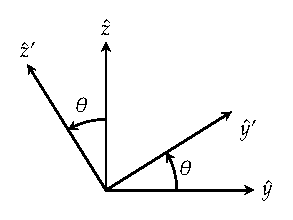
\includegraphics{fig_ch2_prob_axes_rotation.pdf}
	\caption{The $y$ and $z$ axes and the axes $y'$ and $z'$ turned by $\theta$ about the $x$ axis.}
	\label{co:fig:axes_rotation}
\end{figure}

\paragraph{What a turn about the pole does to a star.} Apply $\mathbf R_z(\theta)$ to the equatorial column \eqref{eq:unit_vector_eq},
\begin{align}
	\mathbf R_z(\theta)\,\hat{\mathbf r}_{\rm eq}
	&\eqby{1} \begin{pmatrix}\cos\delta\cos\alpha\cos\theta+\cos\delta\sin\alpha\sin\theta\\ -\cos\delta\cos\alpha\sin\theta+\cos\delta\sin\alpha\cos\theta\\ \sin\delta\end{pmatrix} \nonumber\\
	&\eqby{2} \begin{pmatrix}\cos\delta\cos(\alpha-\theta)\\ \cos\delta\sin(\alpha-\theta)\\ \sin\delta\end{pmatrix}.
	\label{co:eq:rz_shift}
\end{align}
\begin{explain}
	\item Each row of Eq.~\eqref{eq:z_axis_rotation_matrix} times the column.
	\item The angle-difference identities.
\end{explain}
A turn by $\theta$ about the pole subtracts $\theta$ from every right ascension and leaves every declination alone.

% ==============================================================================
\section{Horizontal Coordinates}
\label{co:sec:horizontal}

The equatorial frame gives each star a fixed column, Eq.~\eqref{eq:unit_vector_eq}, and Section~\ref{co:sec:rotation} gives the matrix for any change of frame.

A star's $(\alpha,\delta)$ does not say whether the star is above the horizon now, or where to point. That needs a frame tied to the ground.

Think of pointing out an aeroplane to a friend. You say ``thirty degrees up, toward the east-north-east''. One angle is the height above the horizon. The other is the compass direction, counted round from north. Neither needs any knowledge of the sky, only of the ground. The answer changes from minute to minute because the plane moves.

For a star it is the ground that moves. The \textbf{altitude} and \textbf{azimuth} use the zenith as their pole and turn with the Earth. The hour angle measures how far the sky has turned since the star crossed the meridian. The idea is that the horizontal frame is the equatorial frame turned about the pole to the meridian, and then tipped about the east--west line so that the zenith takes the place of the pole.

A star on the celestial equator crossing the meridian of IISER TVM, at latitude $\phi_0=8.68^\circ\mathrm N$, stands at altitude $90^\circ-8.68^\circ=81.32^\circ$, due south. The pole is $8.68^\circ$ above the northern horizon, so the equator, $90^\circ$ from the pole, passes $8.68^\circ$ south of the zenith.

The picture is a dome over flat ground. The zenith is overhead, the horizon is the rim, and the meridian is the arc from the north point through the zenith to the south point.

The east--north--up frame of surveying and of radar is the same frame. The hour angle is the clock of Chapter~\ref{ch:time} read for one star. It gives the matrix between the equatorial and horizontal frames, in both directions.

\paragraph{The angles.} The \textbf{altitude} $h\in[-90^\circ,+90^\circ]$ is the angle of a star above the horizon, $+90^\circ$ at the zenith and $-90^\circ$ at the nadir. The \textbf{zenith angle} is its distance from the zenith,
\begin{equation}
	z = 90^\circ - h.
	\label{eq:zenith_angle_def}
\end{equation}
The \textbf{azimuth} $A\in[0^\circ,360^\circ)$ is the angle along the horizon from north ($0^\circ$) through east ($90^\circ$), south ($180^\circ$) and west ($270^\circ$). The \textbf{hour angle} of Eq.~\eqref{eq:hour_angle_def} is the angle along the celestial equator from the meridian westward to the star's hour circle,
\begin{equation}
	H = \LST - \alpha,
	\label{eq:hour_angle_formula}
\end{equation}
with $H>0$ after the star has crossed the meridian.

\begin{figure}[htbp]
	\centering
	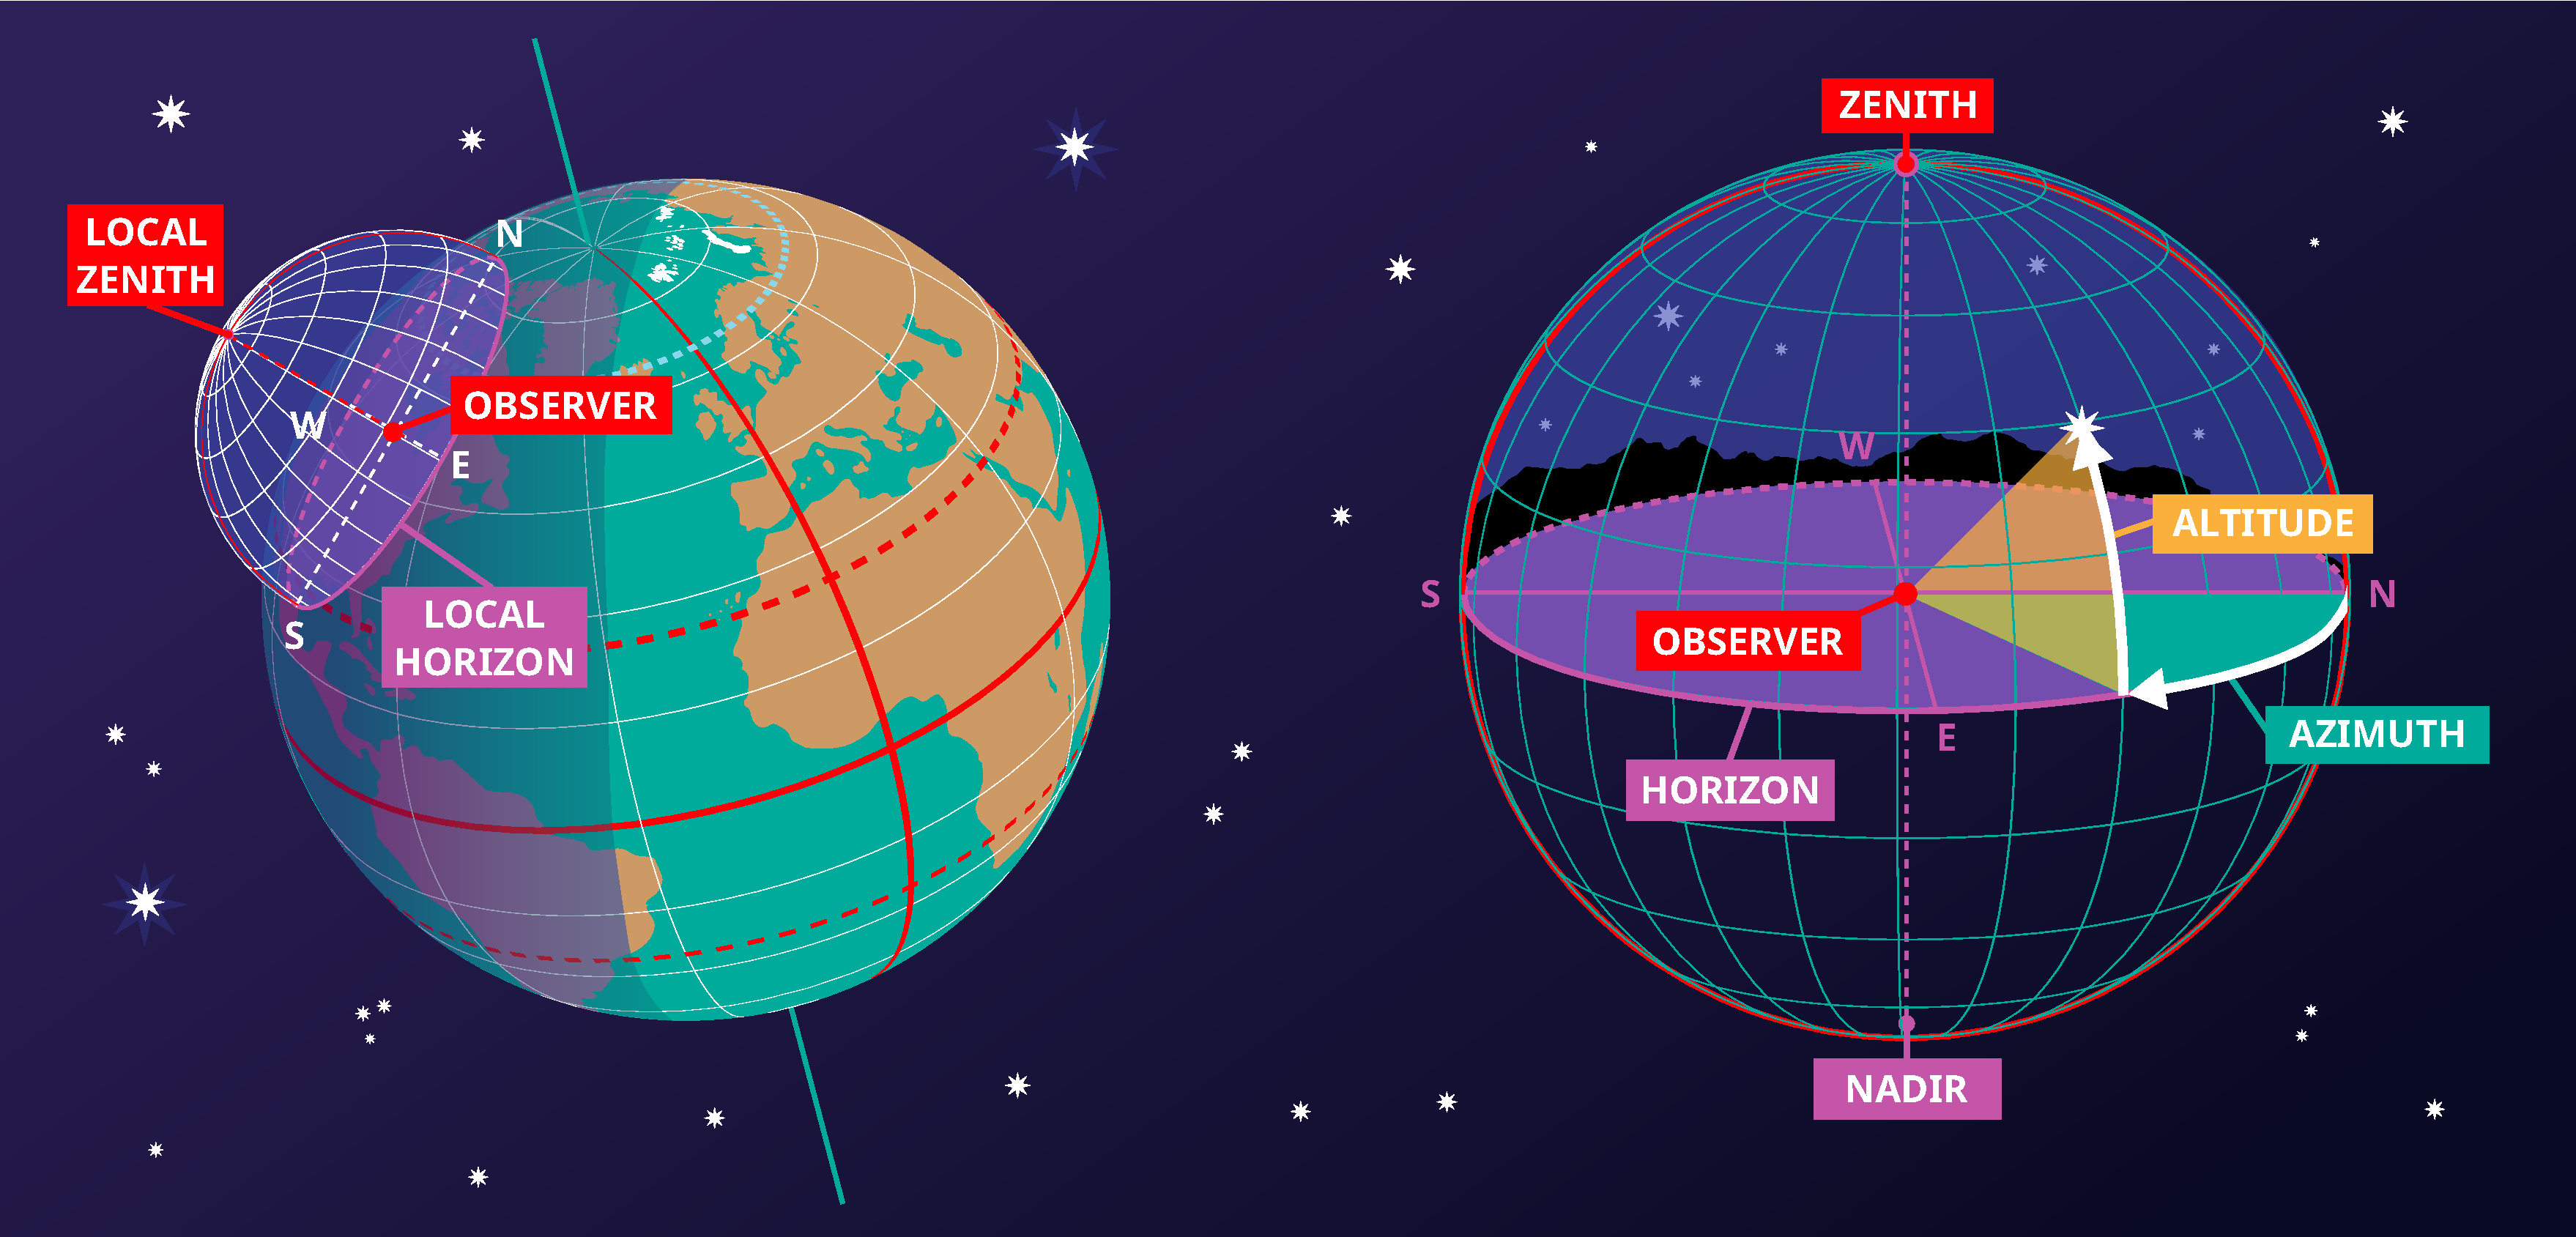
\includegraphics[width=0.75\linewidth]{altitude_azimuth_en.pdf}
	\caption{Left, an observer on the Earth with the local horizon and zenith. Right, the observer's sky with the horizon, zenith, nadir, the cardinal points, and the altitude and azimuth of a star.}
	\label{fig:altaz}
	\label{fig:ch2_prob_alt_az}
\end{figure}

\subsection{The Meridian Frame}

To compare the two systems we first turn the equatorial axes about the pole until the $x$ axis lies in the observer's meridian. The right ascension on the meridian is $\LST$, so the turn is $\mathbf R_z(\LST)$, and Eq.~\eqref{co:eq:rz_shift} gives
\begin{align}
	\hat{\mathbf r}_{\rm mer}
	&\eqby{1} \begin{pmatrix} \cos\LST & \sin\LST & 0 \\ -\sin\LST & \cos\LST & 0 \\ 0 & 0 & 1 \end{pmatrix}\begin{pmatrix} \cos\delta\cos\alpha \\ \cos\delta\sin\alpha \\ \sin\delta \end{pmatrix}
	\label{eq:meridian_rotation_applied}\\
	&\eqby{2} \begin{pmatrix}\cos\delta\cos(\alpha-\LST) \\ \cos\delta\sin(\alpha-\LST) \\ \sin\delta\end{pmatrix}
	\label{eq:meridian_frame_general}\\
	&\eqby{3} \begin{pmatrix} \cos\delta\cos H \\ -\cos\delta\sin H \\ \sin\delta \end{pmatrix}.
	\label{eq:unit_meridian_frame}
\end{align}
\begin{explain}
	\item Eq.~\eqref{eq:z_axis_rotation_matrix} with $\theta=\LST$, acting on Eq.~\eqref{eq:unit_vector_eq}.
	\item Eq.~\eqref{co:eq:rz_shift}.
	\item $\alpha-\LST=-H$ by Eq.~\eqref{eq:hour_angle_formula}, with $\cos(-H)=\cos H$ and $\sin(-H)=-\sin H$.
\end{explain}
In this frame the $x$ axis points to where the meridian crosses the celestial equator, the $y$ axis points to the east point of the horizon ($H=-90^\circ$, $\delta=0$), and the $z$ axis still points to the pole. The right ascension and the sidereal time now enter only through their difference $H$.

\subsection{The Local Axes}

Next we need the observer's north, east and up directions in the meridian frame.

\paragraph{Up.} The zenith lies on the meridian. Its declination is the latitude $\phi_0$, because the angle between the celestial equator and the zenith is the angle between the Earth's equator and the local vertical. Setting $H=0$ and $\delta=\phi_0$ in Eq.~\eqref{eq:unit_meridian_frame} gives the up direction $\hat{\mathbf u}$.

\paragraph{East.} The east point of the horizon is $90^\circ$ from the zenith and $90^\circ$ from the pole, since it is on the horizon and both the zenith and the pole lie on the meridian. So it lies on the celestial equator, a quarter turn east of the meridian, at $\delta=0$ and $H=-90^\circ$.

\paragraph{North.} North is the horizontal direction that completes the frame, $\hat{\mathbf n}=\hat{\mathbf u}\times\hat{\mathbf e}$. With the two vectors just found,
\begin{align}
	\hat{\mathbf u} &= \begin{pmatrix} \cos\phi_0 \\ 0 \\ \sin\phi_0 \end{pmatrix}, \qquad
	\hat{\mathbf e} = \begin{pmatrix} 0 \\ 1 \\ 0 \end{pmatrix}, \label{eq:basis_z}\\
	\hat{\mathbf n} &= \hat{\mathbf u}\times\hat{\mathbf e}
	\eqby{1} \begin{pmatrix} 0\cdot0-\sin\phi_0\cdot1 \\ \sin\phi_0\cdot0-\cos\phi_0\cdot0 \\ \cos\phi_0\cdot1-0\cdot0 \end{pmatrix}
	= \begin{pmatrix} -\sin\phi_0 \\ 0 \\ \cos\phi_0 \end{pmatrix}. \label{eq:basis_n}
\end{align}
\begin{explain}
	\item The components of a cross product, $(u_ye_z-u_ze_y,\ u_ze_x-u_xe_z,\ u_xe_y-u_ye_x)$.
\end{explain}
A second route gives the same $\hat{\mathbf n}$. The north point is on the meridian, $90^\circ$ beyond the zenith, past the pole. Putting $H=0$ and $\delta=90^\circ+\phi_0$ into Eq.~\eqref{eq:unit_meridian_frame} gives $(\cos(90^\circ+\phi_0),0,\sin(90^\circ+\phi_0))=(-\sin\phi_0,0,\cos\phi_0)$. For later reference the east vector is
\begin{equation}
	\hat{\mathbf e}=(0,1,0)^{T}.
	\label{eq:basis_e}
\end{equation}
The triple $(\hat{\mathbf n},\hat{\mathbf e},\hat{\mathbf u})$ is left-handed, $\hat{\mathbf n}\times\hat{\mathbf e}=-\hat{\mathbf u}$, because the azimuth runs clockwise as seen from above.

\begin{figure}[htbp]
	\centering
	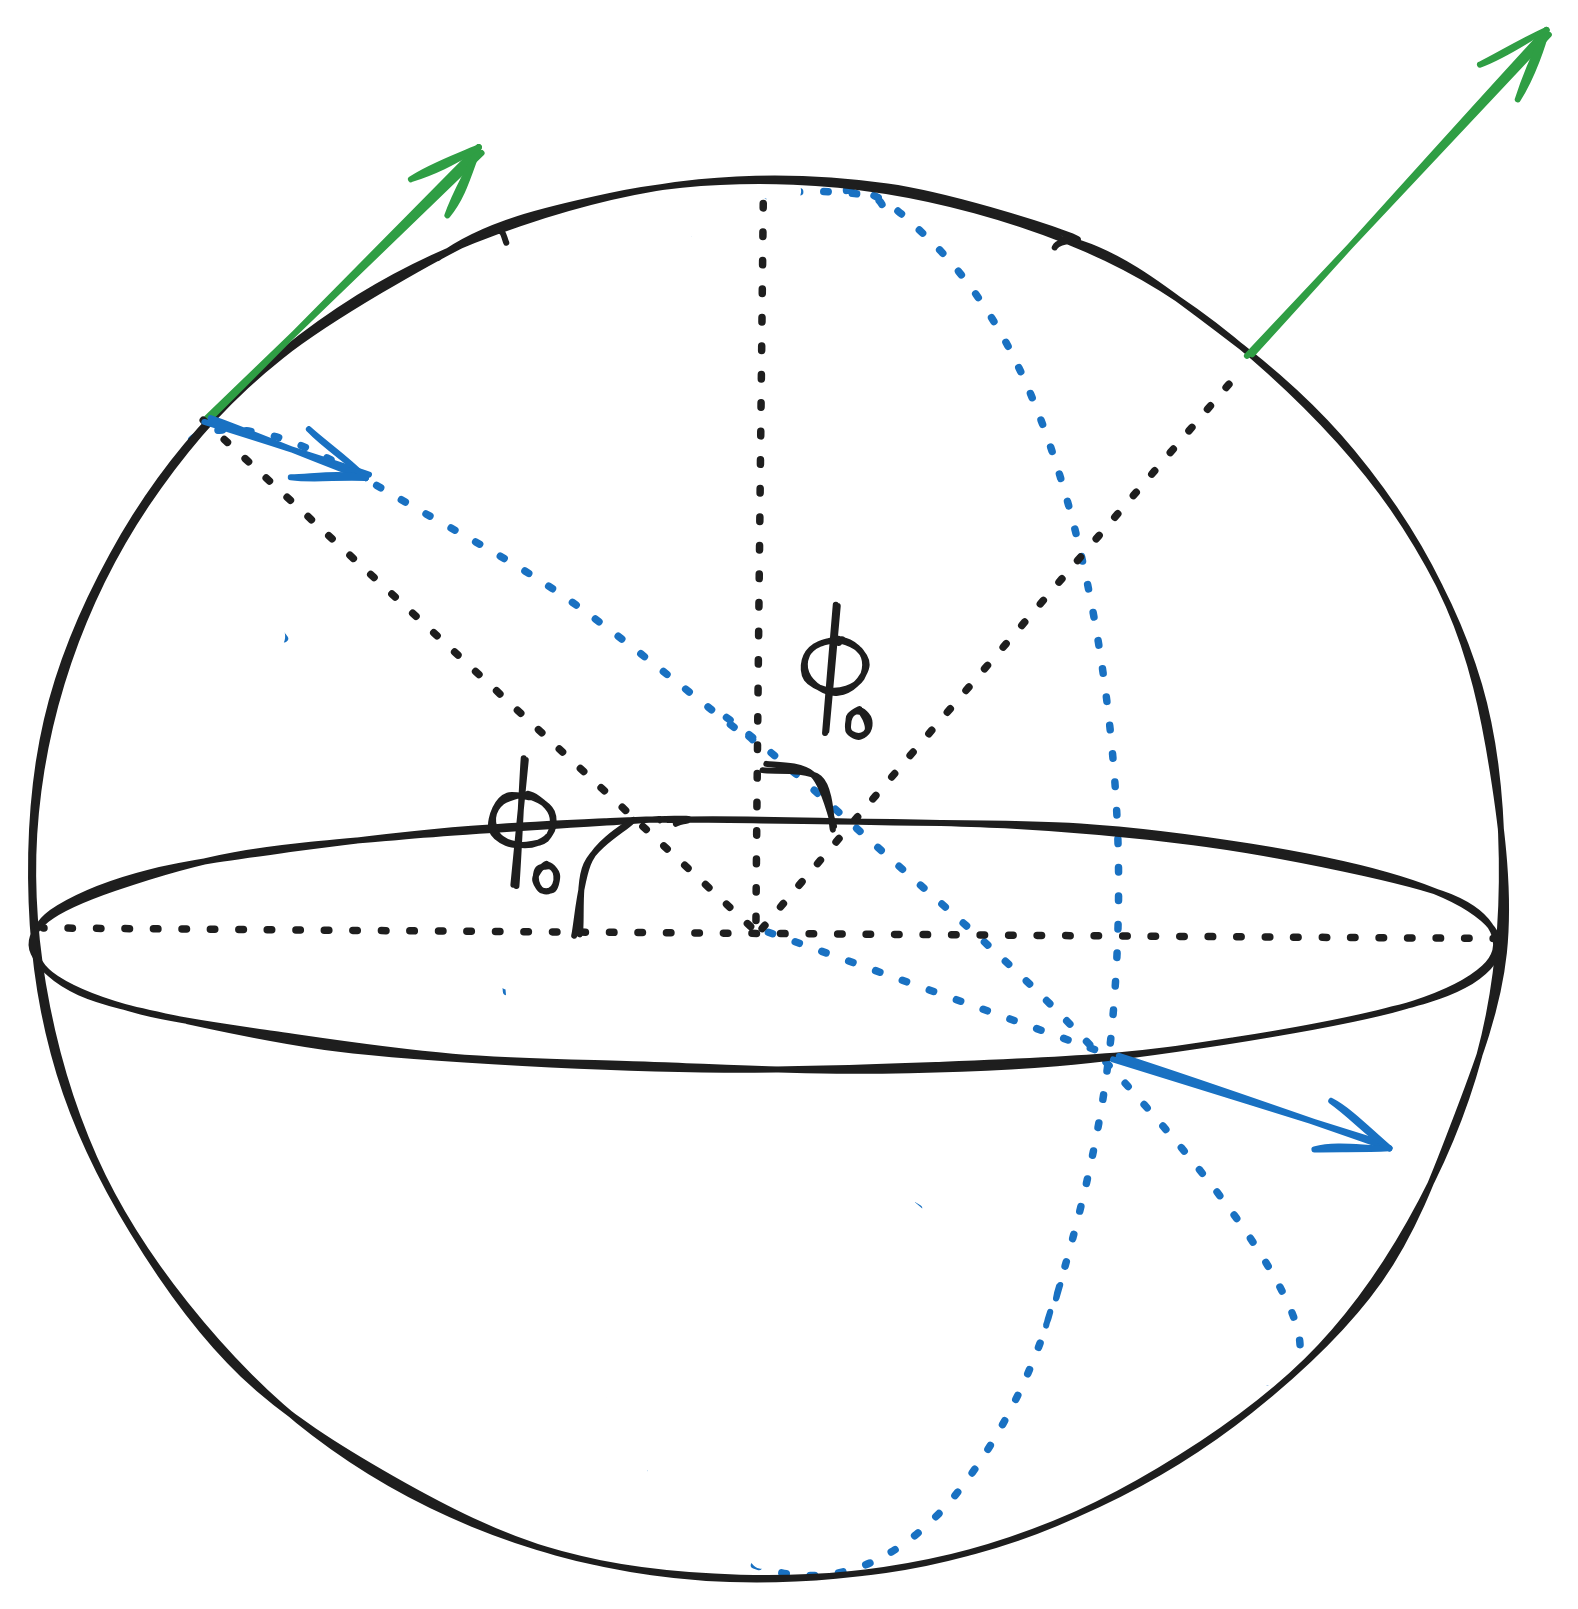
\includegraphics[width=0.4\linewidth]{local north and east.png}
	\caption{The local north (blue) and up (green) directions at an observer at latitude $\phi_0$, drawn on the Earth.}
	\label{fig:local_coordinates}
	\label{fig:ch2_prob_local_coordinates}
\end{figure}

\subsection{The Transformation}

The goal is $(h,A)$ in terms of $(\delta,H)$. A star at altitude $h$ and azimuth $A$ has, by the same split as Eq.~\eqref{eq:unit_vector_eq} with $h$ for $\delta$ and $A$ counted from north,
\begin{equation}
	\hat{\mathbf r}=(\cos h\cos A)\,\hat{\mathbf n}+(\cos h\sin A)\,\hat{\mathbf e}+(\sin h)\,\hat{\mathbf u}.
\end{equation}
In the meridian frame this is a matrix whose columns are the three local axes,
\begin{equation}
	\hat{\mathbf r}_{\rm mer}
	=\begin{pmatrix} \hat{\mathbf n} & \hat{\mathbf e} & \hat{\mathbf u} \end{pmatrix}\hat{\mathbf r}_{\rm hor}
	=\underbrace{\begin{pmatrix}
	\color{colone}{-\sin\phi_0} & \color{coltwo}{0} & \color{colthree}{\cos\phi_0}\\
	\color{colone}{0} & \color{coltwo}{1} & \color{colthree}{0}\\
	\color{colone}{\cos\phi_0} & \color{coltwo}{0} & \color{colthree}{\sin\phi_0}
	\end{pmatrix}}_{\mathbf M(\phi_0)}
	\begin{pmatrix}
	\color{colone}{\cos h\cos A}\\
	\color{coltwo}{\cos h\sin A}\\
	\color{colthree}{\sin h}
	\end{pmatrix}.
	\label{co:eq:hor_columns}
\end{equation}
To solve for the horizontal column we invert $\mathbf M(\phi_0)$,
\begin{align}
	\begin{pmatrix} \cos h\cos A \\ \cos h\sin A \\ \sin h \end{pmatrix}
	&\eqby{1} \mathbf M^{T}(\phi_0)\,\hat{\mathbf r}_{\rm mer} \nonumber\\
	&\eqby{2} \begin{pmatrix} -\sin\phi_0 & 0 & \cos\phi_0 \\ 0 & 1 & 0 \\ \cos\phi_0 & 0 & \sin\phi_0 \end{pmatrix} \begin{pmatrix} \cos\delta\cos H \\ -\cos\delta\sin H \\ \sin\delta \end{pmatrix}
	\label{eq:eq_to_hor_matrix}\\
	&\eqby{3} \begin{pmatrix} -\sin\phi_0\cos\delta\cos H+\cos\phi_0\sin\delta \\ -\cos\delta\sin H \\ \cos\phi_0\cos\delta\cos H+\sin\phi_0\sin\delta \end{pmatrix}. \nonumber
\end{align}
\begin{explain}
	\item The columns of $\mathbf M(\phi_0)$ are orthonormal, so $\mathbf M^{-1}=\mathbf M^{T}$, Eq.~\eqref{co:eq:orthogonal}.
	\item $\mathbf M(\phi_0)$ is symmetric, so $\mathbf M^{T}=\mathbf M$. The column $\hat{\mathbf r}_{\rm mer}$ is Eq.~\eqref{eq:unit_meridian_frame}.
	\item Each row times the column.
\end{explain}
Reading off the three rows,
\begin{keyresult}
	\begin{align}
		\sin h &= \sin\phi_0\sin\delta + \cos\phi_0\cos\delta\cos H, \label{eq:sinh_master} \\
		\cos h\sin A &= -\cos\delta\sin H, \label{eq:cosh_sinA} \\
		\cos h\cos A &= -\sin\phi_0\cos\delta\cos H + \cos\phi_0\sin\delta. \label{eq:cosh_cosA}
	\end{align}
\end{keyresult}
The star enters only through $\delta$, the time only through $H$, and the site only through $\phi_0$. The site's longitude enters only through the LST inside $H$. The last row is also $\hat{\mathbf u}\cdot\hat{\mathbf r}=\cos z$, the dot product of the up vector \eqref{eq:basis_z} with Eq.~\eqref{eq:unit_meridian_frame}.

\paragraph{The azimuth.} Dividing Eq.~\eqref{eq:cosh_sinA} by Eq.~\eqref{eq:cosh_cosA},
\begin{equation}
	\tan A = \frac{-\cos\delta\sin H}{-\sin\phi_0\cos\delta\cos H + \cos\phi_0\sin\delta} \eqby{1} \frac{\sin H}{\sin\phi_0\cos H - \cos\phi_0\tan\delta}.
	\label{eq:tanA_master}
\end{equation}
\begin{explain}
	\item Numerator and denominator divided by $-\cos\delta$.
\end{explain}
That division flips the sign of both parts, so the second form cannot tell $A$ from $A+180^\circ$. The quadrant comes from the signs of Eqs.~\eqref{eq:cosh_sinA} and \eqref{eq:cosh_cosA} themselves. $\sin A$ has the sign of $\cos h\sin A$, and $\cos A$ the sign of $\cos h\cos A$, because $\cos h\ge0$.

\paragraph{Going back.} The product of $\mathbf M(\phi_0)$ with itself is
\begin{equation}
	\mathbf M(\phi_0)\,\mathbf M(\phi_0)
	=\begin{pmatrix}\sin^2\phi_0+\cos^2\phi_0&0&-\sin\phi_0\cos\phi_0+\cos\phi_0\sin\phi_0\\0&1&0\\-\cos\phi_0\sin\phi_0+\sin\phi_0\cos\phi_0&0&\cos^2\phi_0+\sin^2\phi_0\end{pmatrix}=\Id ,
\end{equation}
so the same matrix also takes horizontal to equatorial coordinates. Eq.~\eqref{co:eq:hor_columns} multiplied out reads
\begin{equation}
	\boxed{\begin{aligned}
	\sin\delta &= \sin\phi_0\sin h + \cos\phi_0\cos h\cos A,\\
	\cos\delta\cos H &= \cos\phi_0\sin h - \sin\phi_0\cos h\cos A,\\
	-\cos\delta\sin H &= \cos h\sin A .
	\end{aligned}}
	\label{co:eq:hor_to_eq}
\end{equation}
These are Eqs.~\eqref{eq:sinh_master}--\eqref{eq:cosh_cosA} with the pairs $(\delta,H)$ and $(h,A)$ exchanged. The reason is that $\mathbf M(\phi_0)$ sends the pole $(0,0,1)^T$ to the zenith $\hat{\mathbf u}$ and the zenith back to the pole, and leaves east alone. It is a mirror, not a rotation. Its determinant is $-\sin^2\phi_0-\cos^2\phi_0=-1$, as it must be for a left-handed set of axes. Tipping the pole onto the zenith about the east--west line would be a rotation. Counting the azimuth clockwise reverses one axis on top of that.

\paragraph{The astronomical triangle.} The pole, the zenith and the star are the corners of a spherical triangle (Figure~\ref{fig:astronomical_triangle}). Its sides are the co-latitude $90^\circ-\phi_0$, the star's distance from the pole $90^\circ-\delta$, and its zenith angle $z$. Its angle at the pole is $H$. For a star west of the meridian its angle at the zenith is $360^\circ-A$. Eq.~\eqref{eq:sinh_master} is the cosine rule of spherical trigonometry for the side $z$. The matrix route gives all three relations at once and with their signs. The third angle, at the star, is the parallactic angle $q$ of Section~\ref{sec:parallactic_angle}.

\begin{figure}[htbp]
	\centering
	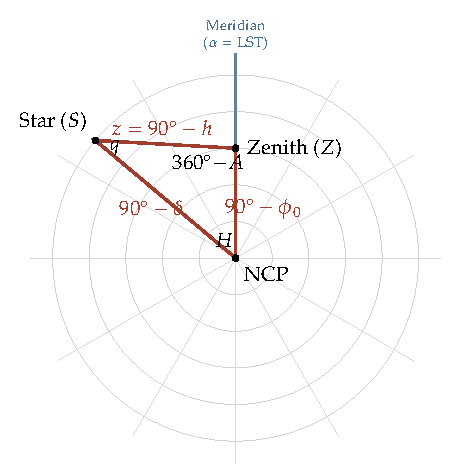
\includegraphics{fig_ch2_horizontal_coords.pdf}
	\caption{The pole--zenith--star triangle for a star west of the meridian, drawn over the equatorial grid near the pole as seen facing north. The sides are $90^\circ-\phi_0$, $90^\circ-\delta$ and $z$. The angles are $H$ at the pole, $360^\circ-A$ at the zenith and $q$ at the star. The sides are drawn straight, though each is an arc of a great circle.}
	\label{fig:astronomical_triangle}
\end{figure}

\paragraph{Worked example, the Sun at an equinox.} At an equinox $\delta_\odot=0$. Three hours after local noon the Sun's hour angle is $H=3^{\rm h}=45^\circ$. At IISER TVM, $\phi_0=8.6833^\circ$, Eqs.~\eqref{eq:sinh_master}--\eqref{eq:cosh_cosA} give
\begin{align}
	\sin h &= \cos(8.6833^\circ)\cos45^\circ = 0.6990, & h&=44.35^\circ, \nonumber\\
	\cos h\sin A &= -\sin45^\circ=-0.7071, \nonumber\\
	\cos h\cos A &= -\sin(8.6833^\circ)\cos45^\circ=-0.1068 . \nonumber
\end{align}
Both $\sin A$ and $\cos A$ are negative, so $A$ is in the third quadrant,
\[
A=180^\circ+\arctan(0.7071/0.1068)=261.41^\circ .
\]
The Sun is $8.59^\circ$ south of due west. At an equinox the Sun runs along the celestial equator, which crosses the horizon at the east and west points and passes south of the zenith at this site. So the Sun stays a little south of the east--west line all day.

% ==============================================================================
\section{Rising, Setting, and Circumpolar Stars}
\label{co:sec:riseset}

Eq.~\eqref{eq:sinh_master} gives the altitude of a star at any hour angle.

To plan a night one wants the reverse, the times when a star is up at all.

Think of a big wheel at a fair whose lower part dips behind a fence. Seats near the hub may never go behind the fence. Seats on the rim spend part of each turn hidden. How much of each turn a seat is hidden depends on its distance from the hub and on how high the fence is compared with the hub.

Each star moves once a sidereal day on a circle of constant $\delta$ around the pole. The horizon cuts that circle, and the height of the pole above the horizon is the latitude. The idea is to set $h=0$ in Eq.~\eqref{eq:sinh_master} and solve for the hour angle.

On the equator, $\phi_0=0$, Eq.~\eqref{eq:sinh_master} reads $\sin h=\cos\delta\cos H$. Every star is on the horizon at $H=\pm90^\circ=\pm6^{\rm h}$, so every star is up for exactly half a sidereal day.

The picture is a set of parallel circles tilted to the horizon by $90^\circ-\phi_0$ and cut by it (Figure~\ref{fig:rising_setting}).

With the Sun's declination in place of the star's, the same formula gives the length of the day, the midnight Sun near the poles and the polar night. It gives the hour angles of rising and setting and the conditions for a star never to set or never to rise.

\paragraph{The rising and setting hour angle.} A star rises or sets when its centre crosses the horizon, $h=0$. In Eq.~\eqref{eq:sinh_master},
\begin{align}
	0 &\eqby{1} \sin\phi_0\sin\delta+\cos\phi_0\cos\delta\cos H_0 , \nonumber\\
	\cos H_0 &\eqby{2} -\frac{\sin\phi_0\sin\delta}{\cos\phi_0\cos\delta} .
\end{align}
\begin{explain}
	\item Eq.~\eqref{eq:sinh_master} with $\sin h=0$.
	\item Divided by $\cos\phi_0\cos\delta$, which is positive away from the poles.
\end{explain}
\begin{equation}
	\boxed{\cos H_0 = -\tan\phi_0\tan\delta.}
	\label{eq:rise_set_master}
\end{equation}
The equation has two roots. The star sets at $H=+H_0$ and rises at $H=-H_0$, with $H_0=\arccos(-\tan\phi_0\tan\delta)$ between $0^\circ$ and $180^\circ$. By Eq.~\eqref{eq:hour_angle_formula} the sidereal times are
\begin{equation}
	\LST_{\rm rise}=\alpha-H_0,\qquad \LST_{\rm set}=\alpha+H_0 .
\end{equation}
The star is up for $2H_0$ of sidereal time. A star north of the equator seen from a northern site has $\tan\phi_0\tan\delta>0$, so $H_0>90^\circ$ and it is up for more than half the day. The formula ignores refraction, which lifts a star on the horizon by about half a degree (Section~\ref{co:sec:refraction}), so a star is seen to rise a little before $-H_0$.

\begin{figure}[htbp]
	\centering
	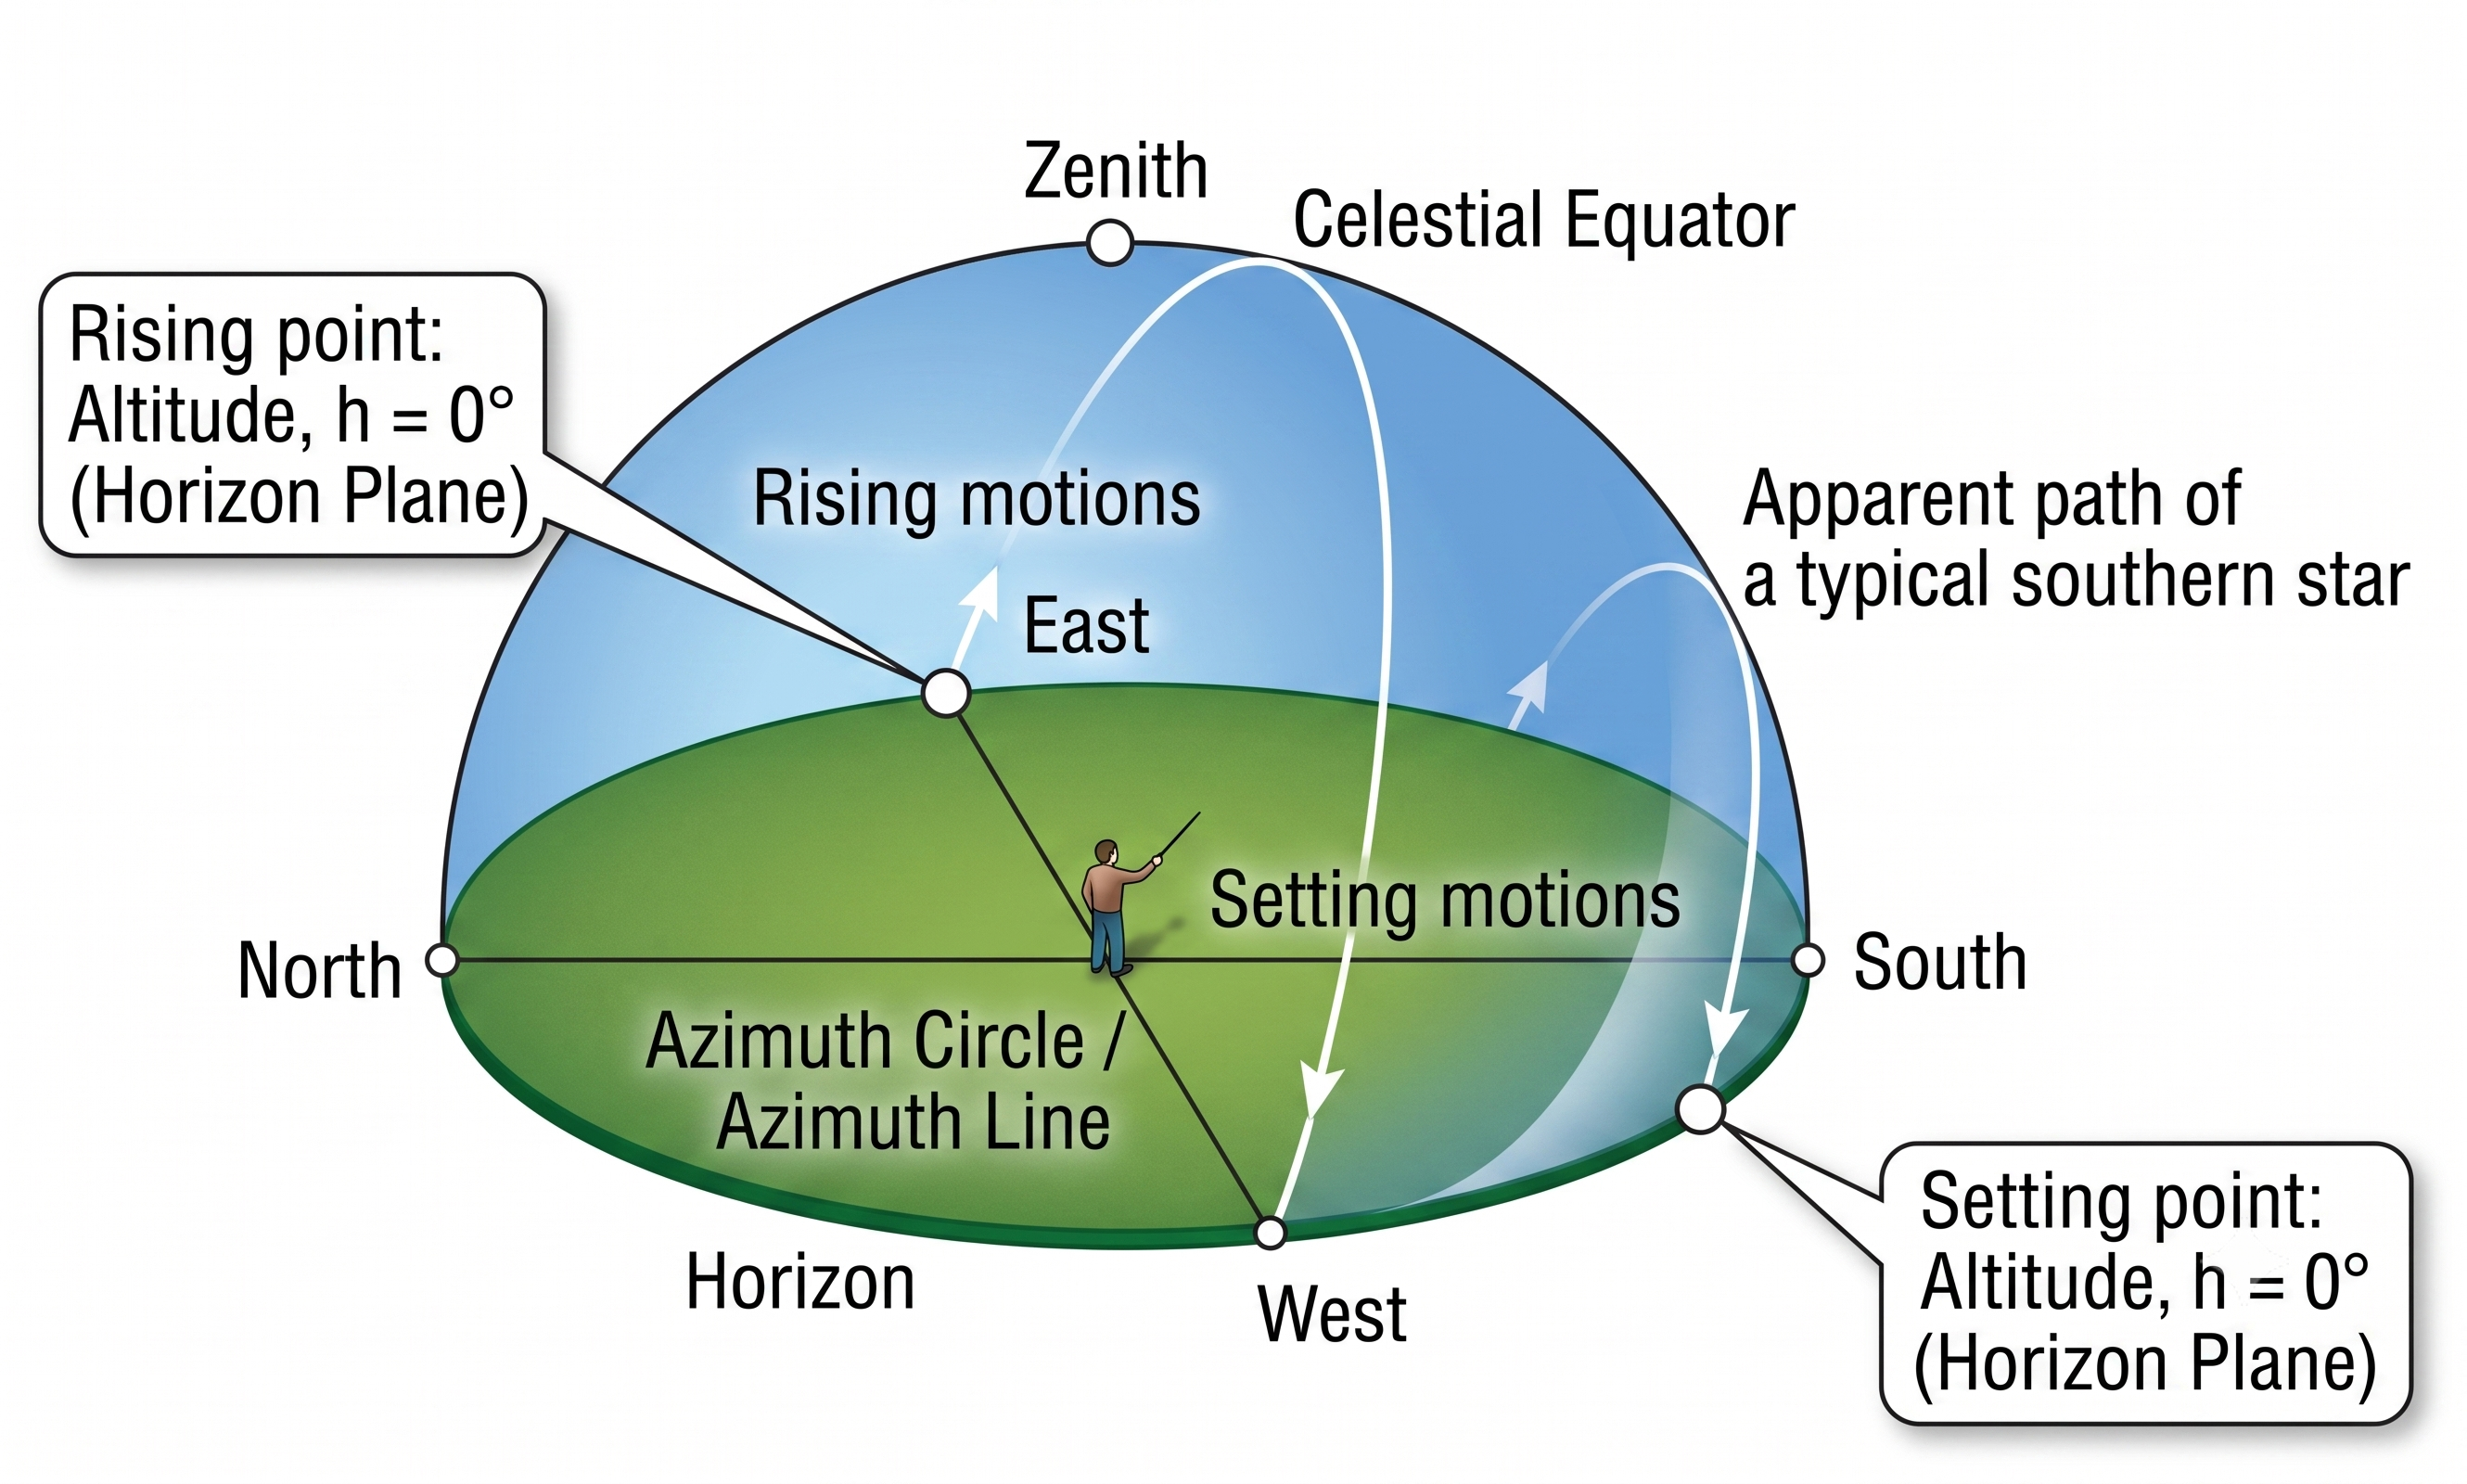
\includegraphics[width=0.55\linewidth]{rising-setting.png}
	\caption{Paths of stars across an observer's sky, with a star rising in the east and setting in the west, and the shorter path of a southern star.}
	\label{fig:rising_setting}
	\label{fig:ch2_prob_rising_setting}
\end{figure}

\paragraph{Stars that never set or never rise.} A root exists only if $|\tan\phi_0\tan\delta|\le1$. Take a northern site, $\phi_0>0$. If $\tan\phi_0\tan\delta>1$ then $\cos H_0<-1$, there is no crossing, and $h>0$ all day. The star is \textbf{circumpolar}. The condition is
\begin{equation}
	\tan\delta \relby{1}{>} \frac{1}{\tan\phi_0}\eqby{2}\tan(90^\circ-\phi_0)
	\quad\Longleftrightarrow\quad \delta>90^\circ-\phi_0 .
	\label{co:eq:circumpolar}
\end{equation}
\begin{explain}
	\item $\tan\phi_0\tan\delta>1$ divided by $\tan\phi_0>0$.
	\item $1/\tan\phi_0=\cot\phi_0=\tan(90^\circ-\phi_0)$. The last step uses that $\tan$ increases on $(-90^\circ,90^\circ)$.
\end{explain}
In the same way a star with $\tan\phi_0\tan\delta<-1$, that is $\delta<-(90^\circ-\phi_0)$, never rises. For a southern site the roles of the two poles swap.

A second route checks the condition. The star is lowest at lower transit, $H=180^\circ$, where Eq.~\eqref{eq:sinh_master} gives
\begin{equation}
	\sin h_{\rm low}=\sin\phi_0\sin\delta-\cos\phi_0\cos\delta\eqby{1}-\cos(\phi_0+\delta)\eqby{2}\sin(\phi_0+\delta-90^\circ),
\end{equation}
\begin{explain}
	\item The angle-sum identity for the cosine.
	\item $-\cos x=\sin(x-90^\circ)$.
\end{explain}
so $h_{\rm low}=\phi_0+\delta-90^\circ$. This is above the horizon exactly when $\delta>90^\circ-\phi_0$, as in Eq.~\eqref{co:eq:circumpolar}.

From IISER TVM, $90^\circ-\phi_0=81.32^\circ$. Polaris, at $\delta=+89.26^\circ$, is circumpolar. It circles the pole between $h_{\rm low}=8.68^\circ+89.26^\circ-90^\circ=7.95^\circ$ and $9.42^\circ$, low in the north all night.

% ==============================================================================
\section{Altitude at Meridian Transit}
\label{co:sec:transit}

Eq.~\eqref{eq:sinh_master} gives the altitude at any hour angle. A star is highest when it crosses the meridian, at $H=0$. That is the best moment to observe it, and for the Sun it is local noon. On the meridian the pole, the zenith and the star lie on one great circle. The zenith is the point of that circle at declination $\phi_0$, so the zenith angle is just the difference of two declinations, as the distance between two towns on one meridian of the Earth is the difference of their latitudes. Chapter~\ref{ch:time} used this for the noon Sun at IISER TVM in its problem set.

\paragraph{The highest altitude.} Put $H=0$ in Eq.~\eqref{eq:sinh_master},
\begin{align}
	\sin h_{\rm max}
	&\eqby{1} \sin\phi_0\sin\delta+\cos\phi_0\cos\delta \nonumber\\
	&\eqby{2} \cos(\phi_0-\delta) \nonumber\\
	&\eqby{3} \sin\big(90^\circ-|\phi_0-\delta|\big).
\end{align}
\begin{explain}
	\item $\cos H=1$.
	\item The angle-difference identity for the cosine.
	\item The cosine is even, so $\cos(\phi_0-\delta)=\cos|\phi_0-\delta|$, and $\cos x=\sin(90^\circ-x)$.
\end{explain}
Both $h_{\rm max}$ and $90^\circ-|\phi_0-\delta|$ lie between $-90^\circ$ and $90^\circ$, so they are equal, and by Eq.~\eqref{eq:zenith_angle_def}
\begin{equation}
	\boxed{z_{\rm min} = |\phi_0 - \delta|.}
	\label{eq:zenith_angle_noon}
\end{equation}
The star crosses south of the zenith if $\delta<\phi_0$ and north of it if $\delta>\phi_0$. At local solar noon the Sun is on the meridian, so its zenith angle is $z_{\rm noon}=|\phi_0-\delta_\odot|$.

\paragraph{Worked example, the June solstice at IISER TVM.} At the June solstice $\delta_\odot=+23.44^\circ$. With $\phi_0=8.6833^\circ\mathrm N$,
\[
z_{\rm noon} = |8.6833^\circ - 23.44^\circ| = 14.76^\circ .
\]
Since $\delta_\odot>\phi_0$, the noon Sun is $14.76^\circ$ north of the zenith.

% ==============================================================================
\section{Angular Distance on the Sphere}
\label{co:sec:angdist}

Each star has a unit vector, Eq.~\eqref{eq:unit_vector_eq}.

The angle between two stars is not found by subtracting their coordinates. Near the pole, two stars $12^{\rm h}$ apart in right ascension can be only a few degrees apart on the sky.

Think of two towns at latitude $60^\circ\mathrm N$ on opposite sides of the globe, $180^\circ$ apart in longitude. Walking west along the parallel covers $180^\circ\times\cos60^\circ=90^\circ$ of arc. Going straight over the pole covers only $30^\circ+30^\circ=60^\circ$. The shortest way is the great circle, and its angle is the angle between the two arrows from the centre of the Earth.

Two stars are two such arrows. The idea is that the cosine of the angle between them is the dot product of their unit vectors.

For the two towns, with $\delta_1=\delta_2=60^\circ$ and $\alpha_1-\alpha_2=180^\circ$, the formula derived below gives $\cos\theta=\sin^260^\circ+\cos^260^\circ\cos180^\circ=0.75-0.25=0.5$, so $\theta=60^\circ$, the route over the pole.

The picture is two arrows from the centre of a ball, with the short arc between their tips.

In navigation this is the great-circle distance, and in spherical trigonometry it is the cosine rule. The scattering angle between two directions in physics is found the same way. It gives the separation of two stars, a form of it that keeps its accuracy for small angles, and the small-angle limit used for proper motions.

\paragraph{The cosine rule.} For two unit vectors, $\cos\theta=\hat{\mathbf r}_1\cdot\hat{\mathbf r}_2$. With Eq.~\eqref{eq:unit_vector_eq},
\begin{align}
	\cos\theta
	&\eqby{1} (\cos\delta_1\cos\alpha_1)(\cos\delta_2\cos\alpha_2) + (\cos\delta_1\sin\alpha_1)(\cos\delta_2\sin\alpha_2) + \sin\delta_1\sin\delta_2 \nonumber \\
	&\eqby{2} \cos\delta_1\cos\delta_2\big(\cos\alpha_1\cos\alpha_2 + \sin\alpha_1\sin\alpha_2\big) + \sin\delta_1\sin\delta_2 \nonumber\\
	&\eqby{3} \sin\delta_1\sin\delta_2 + \cos\delta_1\cos\delta_2\cos(\alpha_1 - \alpha_2).
\end{align}
\begin{explain}
	\item The dot product of the two columns \eqref{eq:unit_vector_eq}, component by component.
	\item $\cos\delta_1\cos\delta_2$ taken out of the first two terms.
	\item The angle-difference identity for the cosine.
\end{explain}
\begin{keyresult}
	\begin{equation}
		\cos\theta = \hat{\mathbf r}_1 \cdot \hat{\mathbf r}_2 = \sin\delta_1\sin\delta_2 + \cos\delta_1\cos\delta_2\cos(\alpha_1 - \alpha_2).
		\label{eq:spherical_law_cos}
	\end{equation}
\end{keyresult}
The result depends on the right ascensions only through their difference, as it must, since a turn about the pole changes neither the angle between two stars nor that difference.

\paragraph{Small angles.} For close pairs Eq.~\eqref{eq:spherical_law_cos} loses accuracy. Then $\cos\theta\approx1-\theta^2/2$, and $\theta$ comes from the small difference of numbers close to one. A computer stores numbers with a relative error of about $10^{-16}$, so $\theta^2/2$ is lost once $\theta$ is below about $1.5\times10^{-8}\,\mathrm{rad}$, which is $3$ milliarcseconds. The cure is to compute $1-\cos\theta=2\sin^2(\theta/2)$ directly,
\begin{align}
	2\sin^2\frac{\theta}{2}
	&\eqby{1} 1-\sin\delta_1\sin\delta_2-\cos\delta_1\cos\delta_2\cos(\alpha_2-\alpha_1) \nonumber\\
	&\eqby{2} 1-\sin\delta_1\sin\delta_2-\cos\delta_1\cos\delta_2+2\cos\delta_1\cos\delta_2\sin^2\frac{\alpha_2-\alpha_1}{2} \nonumber\\
	&\eqby{3} 1-\cos(\delta_2-\delta_1)+2\cos\delta_1\cos\delta_2\sin^2\frac{\alpha_2-\alpha_1}{2} \nonumber\\
	&\eqby{4} 2\sin^2\frac{\delta_2-\delta_1}{2}+2\cos\delta_1\cos\delta_2\sin^2\frac{\alpha_2-\alpha_1}{2}.
\end{align}
\begin{explain}
	\item $1-\cos\theta=2\sin^2(\theta/2)$, with $\cos\theta$ from Eq.~\eqref{eq:spherical_law_cos}.
	\item $\cos x=1-2\sin^2(x/2)$ for $x=\alpha_2-\alpha_1$.
	\item The angle-difference identity, $\cos\delta_1\cos\delta_2+\sin\delta_1\sin\delta_2=\cos(\delta_2-\delta_1)$.
	\item $1-\cos x=2\sin^2(x/2)$ again, for $x=\delta_2-\delta_1$.
\end{explain}
Dividing by two gives the \textbf{haversine formula},
\begin{equation}
	\sin^2\left(\frac{\theta}{2}\right) = \sin^2\left(\frac{\delta_2 - \delta_1}{2}\right) + \cos\delta_1\cos\delta_2\sin^2\left(\frac{\alpha_2 - \alpha_1}{2}\right).
	\label{eq:haversine_formula}
\end{equation}
Every term is now small when the stars are close, so nothing is lost.

\paragraph{The flat-sky limit.} For small separations each sine equals its argument. Writing $\Delta\delta=\delta_2-\delta_1$ and $\Delta\alpha=\alpha_2-\alpha_1$, and keeping the lowest order,
\begin{equation}
	\boxed{\theta^2\approx\Delta\delta^2+\cos^2\delta\,\Delta\alpha^2 .}
	\label{co:eq:flat_sky}
\end{equation}
A step in right ascension is shortened on the sky by $\cos\delta$, because the hour circles crowd together toward the pole. This is why the proper motion in right ascension carries the factor $\cos\delta$ in Eq.~\eqref{eq:total_proper_motion}.

% ==============================================================================
\section{The Ecliptic Coordinate System}
\label{co:sec:ecliptic}

Section~\ref{co:sec:rotation} gives the matrix for a turn about any axis.

The Sun and the planets move close to the ecliptic, which is tilted to the celestial equator. In equatorial coordinates the Sun's declination swings between $-23.44^\circ$ and $+23.44^\circ$ every year. A frame whose equator is the ecliptic removes that swing.

Think of a model railway laid on a tilted table. Measured from the floor, the train rises and falls as it goes round. Measured from the table top, it stays at height zero. Choosing the table as the reference plane removes the rising and falling.

The ecliptic is the table, tilted by the obliquity $\epsilon=23.44^\circ$, and the Sun is the train. In ecliptic coordinates its latitude is always zero. The idea is that the ecliptic frame is the equatorial frame turned by $\epsilon$ about the line to $\hat\gamma$, which lies in both planes.

At the June solstice the Sun is at ecliptic longitude $90^\circ$, a quarter of the way round from $\hat\gamma$. That is where the tilted table stands highest above the floor, so the Sun's declination is the full tilt, $\delta_\odot=+\epsilon=+23.44^\circ$, at $\alpha=6^{\rm h}$.

The picture is two great circles that cross at $\hat\gamma$ at the angle $\epsilon$ (Figure~\ref{fig:equator_elliptic}).

The ecliptic is the plane of the Earth's orbit, so $\epsilon$ is the inclination of the Earth's equator to its orbit. The turn is the same $\mathbf R_x$ that tilted an orbital plane by its inclination in Chapter~\ref{ch:twobody}, Eq.~\eqref{eq:orbital_frame_rotation}. It gives the transformation in both directions and the Sun's declination through the year.

\paragraph{The angles.} The \textbf{ecliptic longitude} $\lambda\in[0^\circ,360^\circ)$ is measured eastward along the ecliptic from $\hat\gamma$. The \textbf{ecliptic latitude} $\beta\in[-90^\circ,+90^\circ]$ is the angle north or south of the ecliptic (Figure~\ref{co:fig:ecliptic_coords}). By the split of Eq.~\eqref{eq:unit_vector_eq}, a star has the ecliptic column
\[
\hat{\mathbf r}_{\rm ecl}=(\cos\beta\cos\lambda,\ \cos\beta\sin\lambda,\ \sin\beta)^{T}.
\]

\begin{figure}[htbp]
	\centering
	\begin{minipage}[c]{0.48\textwidth}
		\centering
		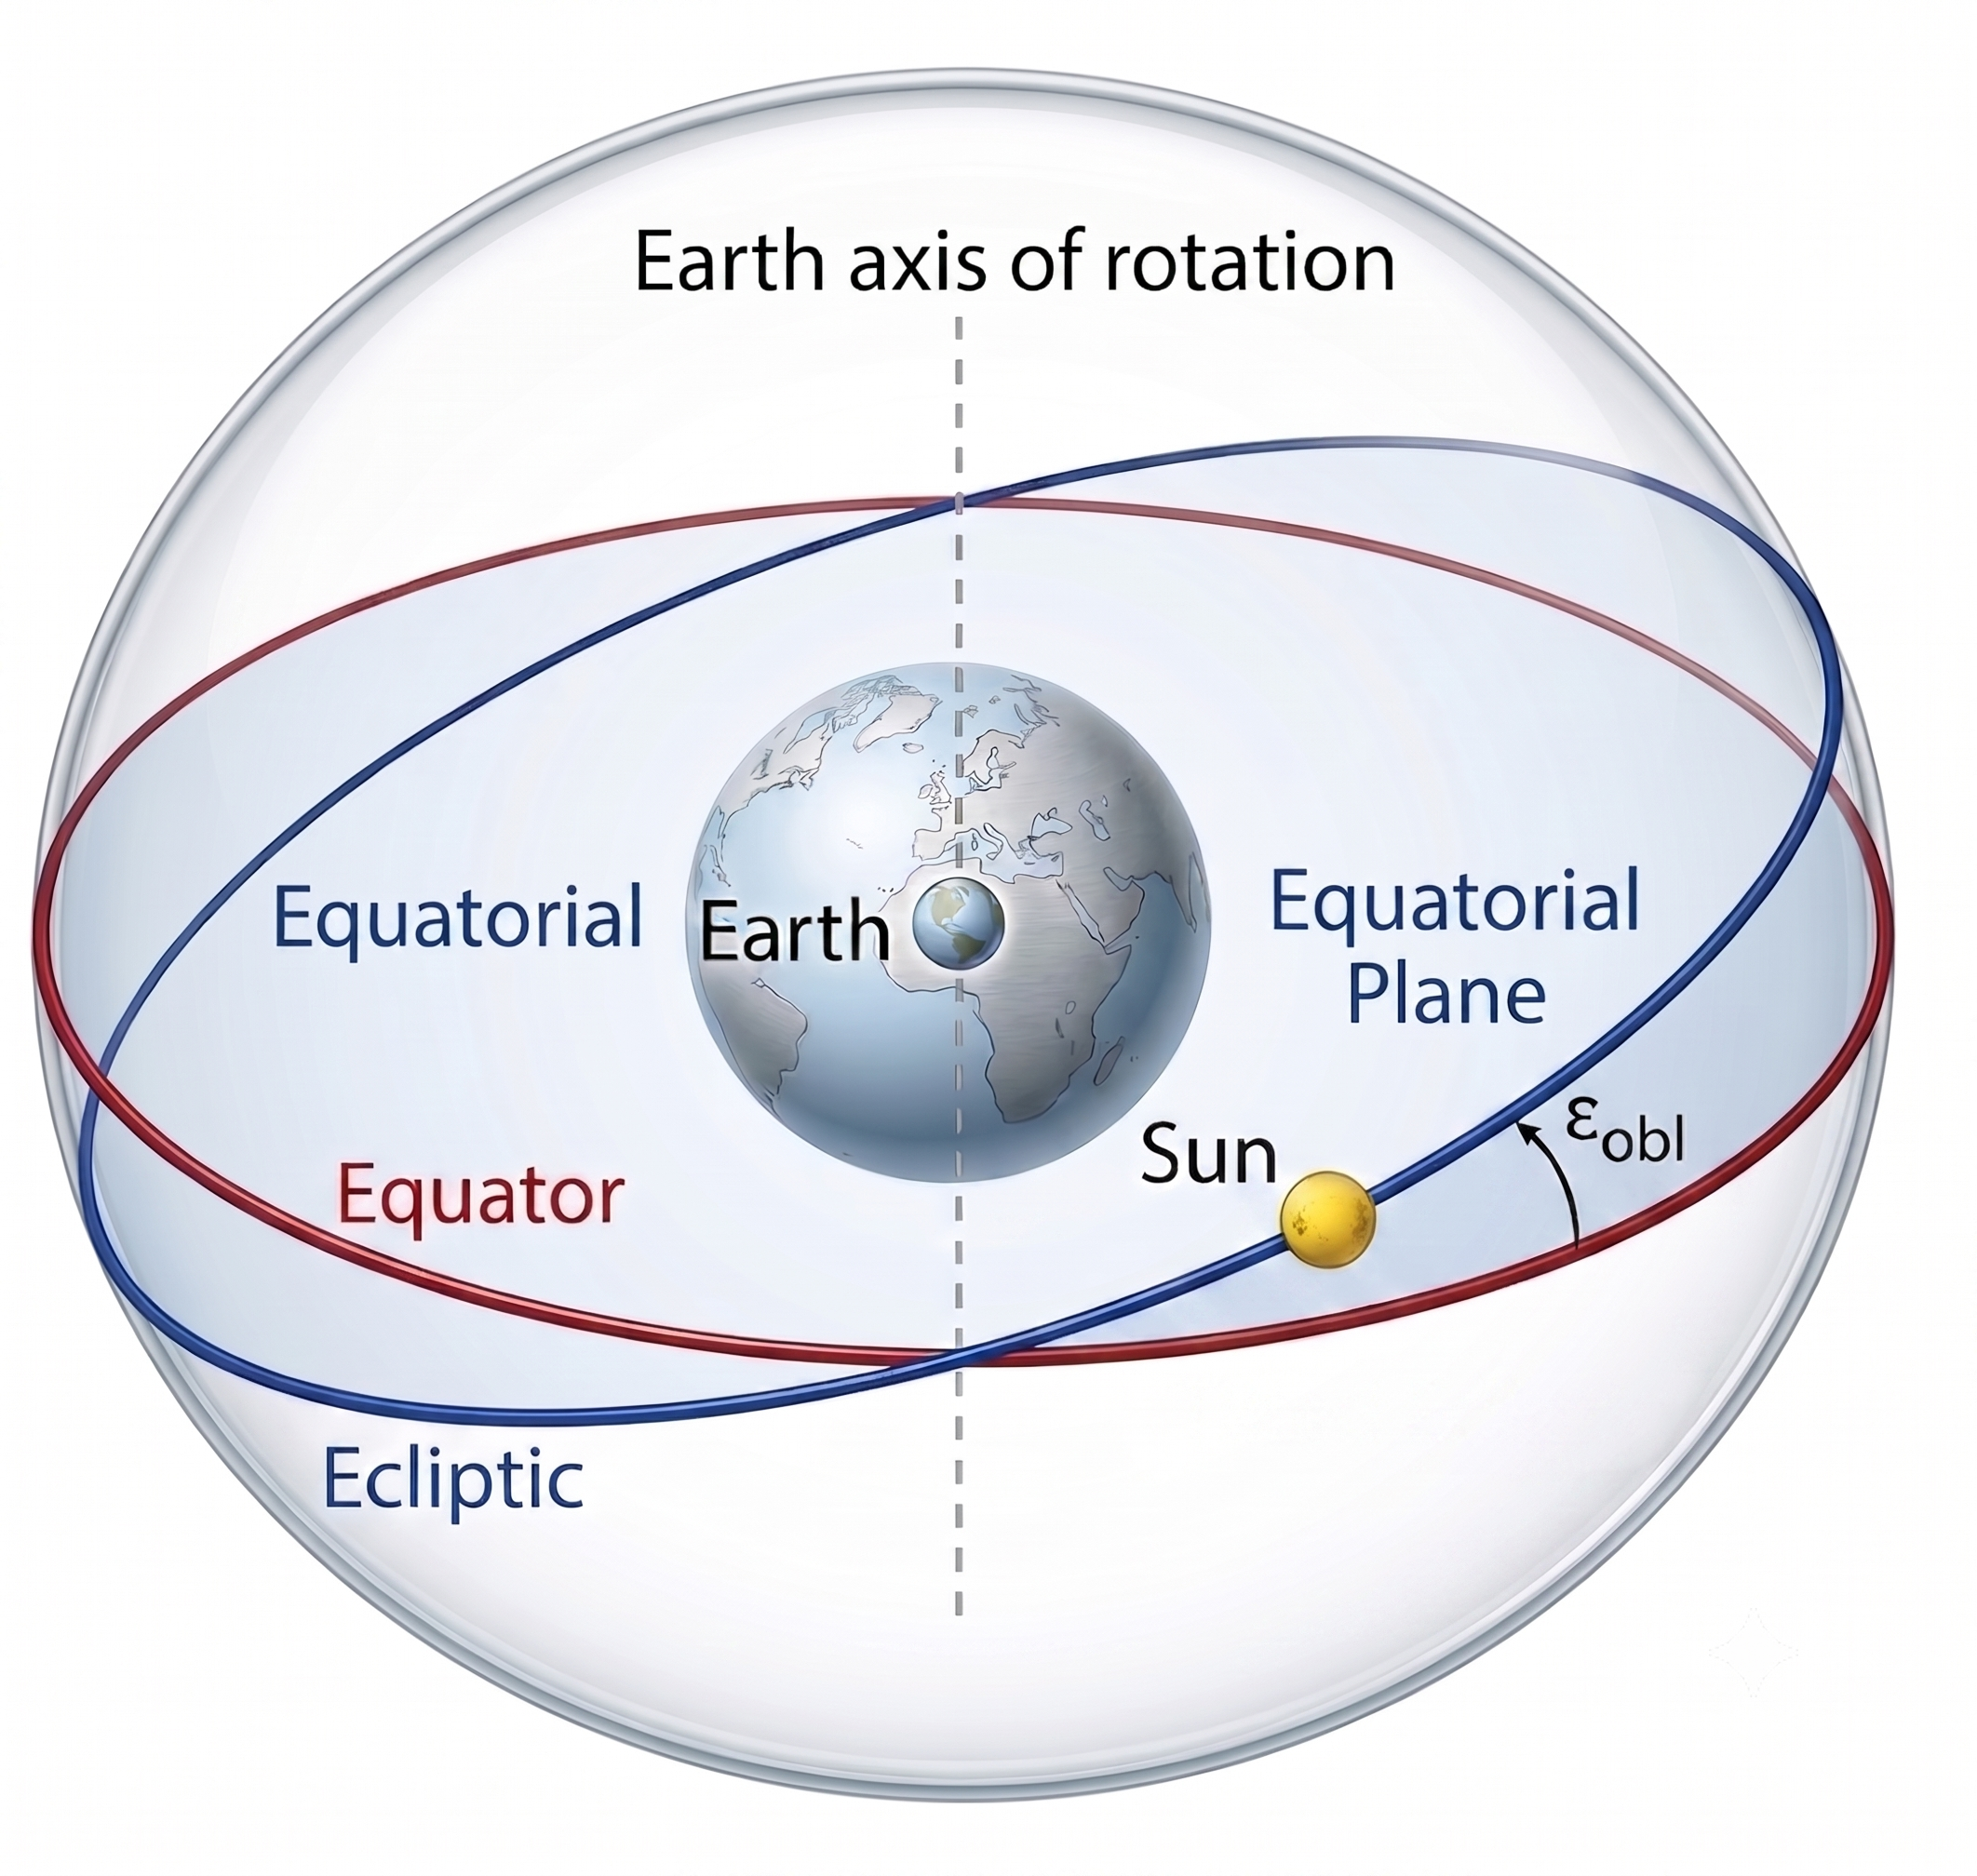
\includegraphics[width=0.85\linewidth]{Equator-Elliptic.png}
		\caption{The celestial equator and the ecliptic around the Earth, crossing at the obliquity $\epsilon\simeq23.44^\circ$.}
		\label{fig:equator_elliptic}
		\label{fig:ch2_prob_equator_elliptic}
	\end{minipage}
	\hfill
	\begin{minipage}[c]{0.48\textwidth}
		\centering
		\resizebox{\linewidth}{!}{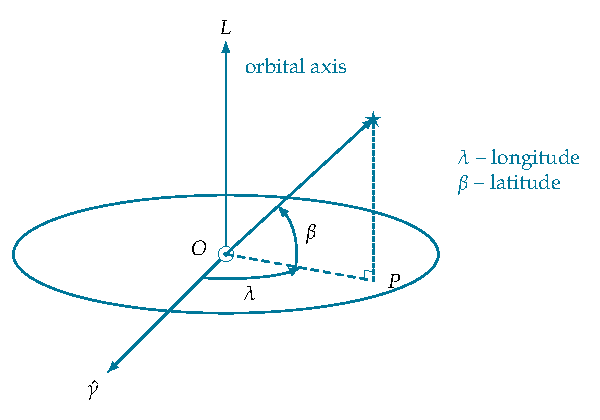
\includegraphics{fig_ch2_prob_ecliptic_coords.pdf}}
		\caption{Ecliptic longitude $\lambda$, measured from $\hat\gamma$ in the ecliptic plane, and ecliptic latitude $\beta$, measured from that plane toward the orbital axis.}
		\label{co:fig:ecliptic_coords}
	\end{minipage}
\end{figure}

\paragraph{The ecliptic axes in equatorial components.} The vernal equinox is on both circles (Section~\ref{sec:sun_coordinates}), so both frames share $\hat{\mathbf x}$. The June solstice point is on the ecliptic at $\alpha=90^\circ$, $\delta=\epsilon$, so its column \eqref{eq:unit_vector_eq} is $(0,\cos\epsilon,\sin\epsilon)^T$. The ecliptic pole is at right angles to both, so it is their cross product, and the third axis completes the set,
\begin{align}
	\hat{\mathbf z}_{\rm ecl}
	&\eqby{1} \hat{\mathbf x}\times\begin{pmatrix}0\\ \cos\epsilon\\ \sin\epsilon\end{pmatrix}
	= \begin{pmatrix}0\cdot\sin\epsilon-0\cdot\cos\epsilon\\ 0\cdot0-1\cdot\sin\epsilon\\ 1\cdot\cos\epsilon-0\cdot0\end{pmatrix}
	= \begin{pmatrix}0\\-\sin\epsilon\\ \cos\epsilon\end{pmatrix}, \nonumber\\
	\hat{\mathbf y}_{\rm ecl}
	&\eqby{2} \hat{\mathbf z}_{\rm ecl}\times\hat{\mathbf x}
	= \begin{pmatrix}-\sin\epsilon\cdot0-\cos\epsilon\cdot0\\ \cos\epsilon\cdot1-0\cdot0\\ 0\cdot0-(-\sin\epsilon)\cdot1\end{pmatrix}
	= \begin{pmatrix}0\\ \cos\epsilon\\ \sin\epsilon\end{pmatrix}.
\end{align}
\begin{explain}
	\item The pole of the ecliptic is perpendicular to every direction in the ecliptic, here $\hat{\mathbf x}$ and the solstice. The order of the factors puts it on the north side, $\cos\epsilon>0$.
	\item A right-handed set has $\hat{\mathbf y}=\hat{\mathbf z}\times\hat{\mathbf x}$.
\end{explain}
The ecliptic $y$ axis points to the solstice, $\lambda=90^\circ$, as it should. The ecliptic pole lies at $\alpha=18^{\rm h}$ and $\delta=90^\circ-\epsilon$.

\paragraph{The transformation.} Stacking $\hat{\mathbf x}$, $\hat{\mathbf y}_{\rm ecl}$ and $\hat{\mathbf z}_{\rm ecl}$ as rows, by Eq.~\eqref{co:eq:rows_rule}, gives exactly $\mathbf R_x(\epsilon)$ of Eq.~\eqref{co:eq:Rx},
\begin{align}
	\begin{pmatrix} \cos\beta\cos\lambda \\ \cos\beta\sin\lambda \\ \sin\beta \end{pmatrix}
	&\eqby{1} \begin{pmatrix} 1 & 0 & 0 \\ 0 & \cos\epsilon & \sin\epsilon \\ 0 & -\sin\epsilon & \cos\epsilon \end{pmatrix} \begin{pmatrix} \cos\delta\cos\alpha \\ \cos\delta\sin\alpha \\ \sin\delta \end{pmatrix}
	\label{eq:ecliptic_rotation_matrix}\\
	&\eqby{2} \begin{pmatrix} \cos\delta\cos\alpha \\ \cos\delta\sin\alpha\cos\epsilon+\sin\delta\sin\epsilon \\ -\cos\delta\sin\alpha\sin\epsilon+\sin\delta\cos\epsilon \end{pmatrix}. \nonumber
\end{align}
\begin{explain}
	\item Eq.~\eqref{co:eq:rows_rule} with the ecliptic axes as rows, acting on Eq.~\eqref{eq:unit_vector_eq}.
	\item Each row times the column.
\end{explain}
Row by row,
\begin{keyresult}
	\begin{align}
		\sin\beta &= \sin\delta\cos\epsilon - \cos\delta\sin\alpha\sin\epsilon, \label{eq:ecliptic_beta} \\
		\cos\beta\cos\lambda &= \cos\delta\cos\alpha, \label{eq:ecliptic_coslam} \\
		\cos\beta\sin\lambda &= \cos\delta\sin\alpha\cos\epsilon + \sin\delta\sin\epsilon. \label{eq:ecliptic_sinlam}
	\end{align}
\end{keyresult}
The longitude needs both of the last two rows. Their ratio alone, $\tan\lambda$, cannot tell $\lambda$ from $\lambda+180^\circ$.

\paragraph{Going back, and the Sun's declination.} The inverse is the transpose, Eq.~\eqref{co:eq:orthogonal}, so $\hat{\mathbf r}_{\rm eq}=\mathbf R_x^{T}(\epsilon)\,\hat{\mathbf r}_{\rm ecl}$. For the Sun, $\beta=0$ and $\hat{\mathbf r}_{\rm ecl}=(\cos\lambda_\odot,\sin\lambda_\odot,0)^T$, so
\begin{equation}
	\begin{pmatrix} \cos\delta_\odot\cos\alpha_\odot \\ \cos\delta_\odot\sin\alpha_\odot \\ \sin\delta_\odot \end{pmatrix}
	\eqby{1} \begin{pmatrix} 1 & 0 & 0 \\ 0 & \cos\epsilon & -\sin\epsilon \\ 0 & \sin\epsilon & \cos\epsilon \end{pmatrix}\begin{pmatrix}\cos\lambda_\odot\\ \sin\lambda_\odot\\ 0\end{pmatrix}
	\eqby{2} \begin{pmatrix}\cos\lambda_\odot\\ \cos\epsilon\sin\lambda_\odot\\ \sin\epsilon\sin\lambda_\odot\end{pmatrix}.
\end{equation}
\begin{explain}
	\item The transpose of Eq.~\eqref{co:eq:Rx} with $\theta=\epsilon$.
	\item Each row times the column.
\end{explain}
\begin{equation}
	\boxed{\sin\delta_\odot=\sin\epsilon\,\sin\lambda_\odot .}
	\label{co:eq:sun_declination}
\end{equation}
The Sun's declination follows from its longitude alone. It is zero at the equinoxes, $\lambda_\odot=0^\circ$ and $180^\circ$, and reaches $\pm\epsilon$ at the solstices, which is the table of Section~\ref{sec:sun_coordinates}.

% ==============================================================================
\section{The Galactic Coordinate System}
\label{co:sec:galactic}

The ecliptic frame was one turn about one axis, because the two planes share the line to $\hat\gamma$.

The disk of the Milky Way is tilted by about $63^\circ$ to the celestial equator, and its zero point, the direction of the Galactic centre, does not lie on the line where the two planes cross. One turn is not enough.

Think of a camera on a tripod. Any way the camera can point is reached by three turns of the tripod head. The head pans about the vertical, tilts about a horizontal axis, and then the camera rolls about its own lens axis.

The Galactic frame is reached from the equatorial frame by the same three turns. A pan about the celestial pole brings the $x$ axis to the line where the Galactic equator crosses the celestial equator. A tilt about that line carries the $z$ axis to the north Galactic pole. A roll about the new pole brings the $x$ axis to the Galactic centre. The idea is that the Galactic frame is the equatorial frame turned by three known angles.

In numbers the pan is $282.86^\circ$, the tilt is $62.87^\circ$ and the roll is $-32.93^\circ$. All three come from the pole's position and one longitude, given below.

The picture is the band of the Milky Way as a great circle tilted steeply to the celestial equator and crossing it twice.

Chapter~\ref{ch:twobody} placed an orbit in space by the same turns, the node longitude $\Omega$, the inclination $\iota$ and the argument of periapsis, Eq.~\eqref{eq:orbital_frame_rotation}. In rigid-body mechanics the three angles are the Euler angles. The matrix found here turns stellar velocities into Galactic ones in Chapter~\ref{ch:astrometry}, Eq.~\eqref{eq:uvw_transform}.

\paragraph{The angles and the pole.} The \textbf{Galactic latitude} $b\in[-90^\circ,+90^\circ]$ is the angle north ($+$) or south ($-$) of the Galactic plane. The \textbf{Galactic longitude} $l\in[0^\circ,360^\circ)$ is measured along the Galactic equator from the direction of the Galactic centre, toward the direction of the Galaxy's rotation at $l=90^\circ$. The radio source Sagittarius A*, at the centre, lies within $0.1^\circ$ of $l=b=0$. By IAU convention the north Galactic pole and the longitude of the north celestial pole are fixed at the J2000.0 values
\begin{align}
	\alpha_{\rm GP} &= 12^{\rm h}51^{\rm m}26.28^{\rm s} = 192.85948^\circ, \qquad \delta_{\rm GP} = +27^\circ 07' 41.7'' = +27.12825^\circ, \nonumber\\
	l_{\rm CP} &= 122.93192^\circ .
\end{align}
Here $l_{\rm CP}$ is the Galactic longitude of the north celestial pole.

\paragraph{The three turns.} The Galactic equator is $90^\circ$ from its pole, so it crosses the celestial equator $90^\circ$ from the pole's hour circle, at $\alpha=\alpha_{\rm GP}+90^\circ$. The angle between the two poles is $90^\circ-\delta_{\rm GP}$. In the Galactic frame that crossing is $90^\circ$ from the half circle of longitude $l_{\rm CP}$ that runs through the celestial pole, at $l=l_{\rm CP}-90^\circ=32.93^\circ$, so the last turn is by $-(l_{\rm CP}-90^\circ)$. With Eqs.~\eqref{eq:z_axis_rotation_matrix} and \eqref{co:eq:Rx},
\begin{equation}
	\hat{\mathbf r}_{\rm gal}
	=\mathbf R_z(90^\circ-l_{\rm CP})\,\mathbf R_x(90^\circ-\delta_{\rm GP})\,\mathbf R_z(\alpha_{\rm GP}+90^\circ)\,\hat{\mathbf r}_{\rm eq}.
	\label{co:eq:gal_product}
\end{equation}
We multiply from the right. The first turn is Eq.~\eqref{co:eq:rz_shift} with $\theta=\alpha_{\rm GP}+90^\circ$,
\begin{align}
	\mathbf R_z(\alpha_{\rm GP}+90^\circ)\,\hat{\mathbf r}_{\rm eq}
	&\eqby{1} \begin{pmatrix}\cos\delta\cos(\alpha-\alpha_{\rm GP}-90^\circ)\\ \cos\delta\sin(\alpha-\alpha_{\rm GP}-90^\circ)\\ \sin\delta\end{pmatrix}
	\eqby{2} \begin{pmatrix}\cos\delta\sin(\alpha-\alpha_{\rm GP})\\ -\cos\delta\cos(\alpha-\alpha_{\rm GP})\\ \sin\delta\end{pmatrix}.
\end{align}
\begin{explain}
	\item Eq.~\eqref{co:eq:rz_shift}.
	\item $\cos(x-90^\circ)=\sin x$ and $\sin(x-90^\circ)=-\cos x$.
\end{explain}
The tilt uses $\cos(90^\circ-\delta_{\rm GP})=\sin\delta_{\rm GP}$ and $\sin(90^\circ-\delta_{\rm GP})=\cos\delta_{\rm GP}$,
\begin{align}
	\mathbf R_x(90^\circ-\delta_{\rm GP})\begin{pmatrix}\cos\delta\sin(\alpha-\alpha_{\rm GP})\\ -\cos\delta\cos(\alpha-\alpha_{\rm GP})\\ \sin\delta\end{pmatrix}
	&\eqby{1} \begin{pmatrix}1&0&0\\0&\sin\delta_{\rm GP}&\cos\delta_{\rm GP}\\0&-\cos\delta_{\rm GP}&\sin\delta_{\rm GP}\end{pmatrix}\begin{pmatrix}\cos\delta\sin(\alpha-\alpha_{\rm GP})\\ -\cos\delta\cos(\alpha-\alpha_{\rm GP})\\ \sin\delta\end{pmatrix} \nonumber\\
	&\eqby{2} \begin{pmatrix}\cos\delta\sin(\alpha-\alpha_{\rm GP})\\ \cos\delta_{\rm GP}\sin\delta-\sin\delta_{\rm GP}\cos\delta\cos(\alpha-\alpha_{\rm GP})\\ \sin\delta_{\rm GP}\sin\delta+\cos\delta_{\rm GP}\cos\delta\cos(\alpha-\alpha_{\rm GP})\end{pmatrix}.
\end{align}
\begin{explain}
	\item Eq.~\eqref{co:eq:Rx} with $\theta=90^\circ-\delta_{\rm GP}$.
	\item Each row times the column.
\end{explain}
For the roll it is simpler to move it to the left side. By Eq.~\eqref{co:eq:orthogonal}, $\mathbf R_z^{T}(\theta)=\mathbf R_z(-\theta)$, so the left side of Eq.~\eqref{co:eq:gal_product} times $\mathbf R_z(l_{\rm CP}-90^\circ)$ is
\begin{align}
	\mathbf R_z(l_{\rm CP}-90^\circ)\begin{pmatrix}\cos b\cos l\\ \cos b\sin l\\ \sin b\end{pmatrix}
	&\eqby{1} \begin{pmatrix}\cos b\cos(l-l_{\rm CP}+90^\circ)\\ \cos b\sin(l-l_{\rm CP}+90^\circ)\\ \sin b\end{pmatrix}
	\eqby{2} \begin{pmatrix}\cos b\sin(l_{\rm CP}-l)\\ \cos b\cos(l_{\rm CP}-l)\\ \sin b\end{pmatrix}.
\end{align}
\begin{explain}
	\item Eq.~\eqref{co:eq:rz_shift} with $\theta=l_{\rm CP}-90^\circ$.
	\item $\cos(x+90^\circ)=-\sin x$ and $\sin(x+90^\circ)=\cos x$, with $x=l-l_{\rm CP}$.
\end{explain}
Setting the last two columns equal, row by row,
\begin{keyresult}
	\begin{align}
		\sin b &= \sin\delta_{\rm GP}\sin\delta + \cos\delta_{\rm GP}\cos\delta\cos(\alpha - \alpha_{\rm GP}), \label{eq:gal_b} \\
		\cos b\sin(l_{\rm CP} - l) &= \cos\delta\sin(\alpha - \alpha_{\rm GP}), \label{eq:gal_sinl} \\
		\cos b\cos(l_{\rm CP} - l) &= \cos\delta_{\rm GP}\sin\delta - \sin\delta_{\rm GP}\cos\delta\cos(\alpha - \alpha_{\rm GP}). \label{eq:gal_cosl}
	\end{align}
\end{keyresult}
The latitude depends only on the star's angle from the Galactic pole, since Eq.~\eqref{eq:gal_b} is the cosine rule \eqref{eq:spherical_law_cos} between the star and the pole. The longitude $l$ needs both of the other two rows to fix its quadrant.

\paragraph{The same formulas as for the horizon.} Eqs.~\eqref{eq:gal_b}--\eqref{eq:gal_cosl} are Eqs.~\eqref{eq:sinh_master}--\eqref{eq:cosh_cosA} with the Galactic pole in place of the zenith. Replace $\phi_0$ by $\delta_{\rm GP}$, the hour angle $H$ by $\alpha_{\rm GP}-\alpha$, the altitude by $b$ and the azimuth $A$ by $l_{\rm CP}-l$. The zenith is a pole at declination $\phi_0$ on the meridian, and the Galactic pole is a pole at declination $\delta_{\rm GP}$ on the hour circle $\alpha_{\rm GP}$. The minus sign in $l_{\rm CP}-l$ is there because the azimuth runs clockwise about its pole and $l$ runs anticlockwise.

\paragraph{The numbers.} Multiplying out Eq.~\eqref{co:eq:gal_product} with the values above gives
\begin{equation}
	\hat{\mathbf r}_{\rm gal}=\begin{pmatrix} -0.054876 & -0.873437 & -0.483835 \\ +0.494109 & -0.444830 & +0.746982 \\ -0.867666 & -0.198076 & +0.455984 \end{pmatrix}\hat{\mathbf r}_{\rm eq}.
	\label{co:eq:T_gal}
\end{equation}
By the rule of rows \eqref{co:eq:rows_rule}, the first row is the direction of the Galactic centre in equatorial components, the second is the direction $l=90^\circ$, and the third is the Galactic pole. The third row is $(\cos\delta_{\rm GP}\cos\alpha_{\rm GP},\cos\delta_{\rm GP}\sin\alpha_{\rm GP},\sin\delta_{\rm GP})$, as Eq.~\eqref{eq:unit_vector_eq} requires. The same matrix appears in Eq.~\eqref{eq:uvw_transform}. Two checks follow. The point $\alpha=266.405^\circ$, $\delta=-28.936^\circ$ comes out at $l=0.0002^\circ$, $b=0.0001^\circ$, so it is the zero point of the frame. Sagittarius A*, at $\alpha=17^{\rm h}45^{\rm m}40.04^{\rm s}$, $\delta=-29^\circ00'28.1''$, comes out at $l=359.944^\circ$, $b=-0.046^\circ$.

% ==============================================================================
\section{Atmospheric Refraction and Stellar Aberration}
\label{co:sec:refraction}

Every formula so far gives the true direction of a star from the centre of the Earth.

The direction in which its light arrives at a telescope is not quite that. The air bends the light, and the motion of the Earth tilts it.

Think of a straw in a glass of water. It looks bent where it enters the water, because light changes direction when it crosses into a medium with a different refractive index. Now think of running through rain that falls straight down. The drops seem to come at you from in front, and you tilt your umbrella forward. The faster you run, the more you tilt it.

Starlight entering the air bends toward the vertical, so a star looks higher than it is. Starlight met by the moving Earth seems to come from a little ahead of the Earth's motion. The idea is that refraction lifts a star by $(n-1)\tan z$ and aberration tilts it forward by $v/c$.

With $n-1=2.82\times10^{-4}$ for air, a star at $z=45^\circ$ is lifted by $2.82\times10^{-4}\,\mathrm{rad}=58''$. The Earth moves round the Sun at $v=29.78\,\mathrm{km\,s^{-1}}$, so $v/c=0.99\times10^{-4}$ and the tilt is $20.5''$.

The picture is a ray bending a little at each layer of air, and a stream of slanted raindrops.

Refraction is Snell's law, and it also makes mirages. Aberration is the low-speed limit of the relativistic aberration of light. Both formulas hold only in a range, and that range is set by comparing two lengths (P6). The flat-layer picture of the air works while the height of the air is small compared with the distance over which the ground curves away. These effects are what move a star from its computed place by arcseconds, and near the horizon by half a degree.

\subsection{Atmospheric Refraction}

The goal is the lift $\Delta h=h_{\rm apparent}-h_{\rm true}$, the same as the drop in zenith angle.

\paragraph{Snell's law through many layers.} Let the air be a stack of flat layers with refractive indices $n_1,n_2,\dots$ from the top down to the ground, where $n_k=n$, and let space above have index $1$. A ray from a star at true zenith angle $z$ enters at the top and reaches the ground at the apparent zenith angle $z'$. Snell's law at each boundary gives
\begin{equation}
	\sin z \eqby{1} n_1\sin z_1 \eqby{1} n_2\sin z_2 \eqby{1} \cdots \eqby{1} n\sin z' .
\end{equation}
\begin{explain}
	\item Snell's law at each flat boundary. The boundaries are parallel, so the angle leaving one layer is the angle arriving at the next.
\end{explain}
All the layers in between cancel. For flat layers the bending depends only on the index at the ground, not on how $n$ varies with height.

\paragraph{The lift.} Put $z'=z-\Delta h$ and expand for small $\Delta h$,
\begin{align}
	\sin z &= n\sin(z-\Delta h) \nonumber\\
	&\eqby{1} n\sin z\cos\Delta h-n\cos z\sin\Delta h \nonumber\\
	&\eqby{2} n\sin z-n\,\Delta h\cos z ,
\end{align}
\begin{explain}
	\item The angle-difference identity for the sine.
	\item $\cos\Delta h=1$ and $\sin\Delta h=\Delta h$ to first order in $\Delta h$.
\end{explain}
so that
\begin{equation}
	\Delta h \approx \frac{(n-1)\sin z}{n\cos z} \approx (n-1)\tan z ,
	\label{eq:refraction_derivation}
\end{equation}
using $n\approx1$ in the denominator. The index of air is a measured property. For visible light at $10^\circ\mathrm C$ and $1010\,\mathrm{hPa}$ it is $n-1=2.82\times10^{-4}$. In arcseconds ($1\,\mathrm{rad}=206\,265''$),
\begin{equation}
	\boxed{\Delta h \approx 58.2''\tan z = 58.2''\cot h \qquad (h > 15^\circ).}
	\label{eq:refraction_cot}
\end{equation}
The lift is zero at the zenith and grows toward the horizon. To first order it does not matter whether $z$ is the true or the apparent zenith angle. Since $n-1$ is proportional to the density of the air, which goes as $P/T$, the coefficient $58.2''$ must be scaled by the local pressure and temperature.

\paragraph{When the flat layers fail (P6).} The air thins with a scale height of $8.4\,\mathrm{km}$, Eq.~\eqref{sg:eq:scale_height}. Call it $H_{\rm air}$ here, to keep it apart from the hour angle. A ray at zenith angle $z$ crosses this lowest scale height while covering a horizontal distance $d=H_{\rm air}\tan z$. Over a horizontal distance $d$ the curved ground of radius $R_\oplus$ falls away below a flat plane by
\begin{equation}
	R_\oplus-\sqrt{R_\oplus^2-d^2}\eqby{1}R_\oplus\Big(1-\sqrt{1-d^2/R_\oplus^2}\Big)\eqby{2}\frac{d^2}{2R_\oplus},
\end{equation}
\begin{explain}
	\item $R_\oplus$ taken out of the bracket.
	\item $\sqrt{1-x}\approx1-x/2$ for $x=d^2/R_\oplus^2\ll1$.
\end{explain}
The flat picture holds while this drop is small compared with $H_{\rm air}$ itself. The ratio of the two lengths is
\begin{equation}
	\frac{d^2/(2R_\oplus)}{H_{\rm air}}=\frac{H_{\rm air}\tan^2z}{2R_\oplus}.
	\label{co:eq:flat_ratio}
\end{equation}
With $R_\oplus=6371\,\mathrm{km}$, $2R_\oplus/H_{\rm air}=1517$. The ratio is $0.01$ at $\tan z=3.9$, that is $z=75.6^\circ$ or $h\approx14^\circ$, which is why Eq.~\eqref{eq:refraction_cot} is quoted for $h>15^\circ$. The ratio reaches one at $\tan z=39$, or $z=88.5^\circ$, and there the flat picture fails outright.

\paragraph{Near the horizon.} Close to the horizon an empirical fit is used instead. Bennett (1982) fitted the refraction as a function of the apparent altitude, $\Delta h[\mathrm{arcmin}]\approx1/\tan\big(h_{\rm app}+7.31^\circ/(h_{\rm app}+4.4^\circ)\big)$. Sæmundsson (1986) turned it round to use the true altitude $h$, and added the scaling of $n-1$ with pressure $P$ and temperature $T$,
\begin{equation}
	\Delta h[\text{arcmin}] \approx \frac{1.02}{\tan\!\left(h + \dfrac{10.3^\circ}{h + 5.11^\circ}\right)}\times\left(\frac{P}{1010\,\text{hPa}}\right)\left(\frac{283}{273 + T[^\circ\text{C}]}\right).
	\label{eq:bennett_formula}
\end{equation}
A star whose true position is on the horizon is lifted by $29'$. A star that is seen exactly on the horizon is really $34.5'$ below it, by Bennett's fit at $h_{\rm app}=0$. That is more than the Sun's angular diameter of about $32'$, so when the setting Sun appears to touch the horizon it is already geometrically below it. At $h=45^\circ$ Eq.~\eqref{eq:bennett_formula} gives $1.01'=61''$, close to the $58''$ of Eq.~\eqref{eq:refraction_cot}.

\subsection{Stellar Aberration}

The goal is the shift of a star's apparent direction caused by the observer's velocity $\vec v$.

\paragraph{The general shift.} Light from a star in the direction $\hat{\mathbf r}$ travels with velocity $-c\,\hat{\mathbf r}$ in the frame of the Sun. Since $v\ll c$, Galilean addition of velocities is enough. In the Earth's frame the light moves with velocity $-c\,\hat{\mathbf r}-\vec v$, so it seems to come from the direction of $c\,\hat{\mathbf r}+\vec v$. The apparent direction is
\begin{align}
	\hat{\mathbf r}'
	&= \frac{c\,\hat{\mathbf r}+\vec v}{|c\,\hat{\mathbf r}+\vec v|}
	\eqby{1} \frac{\hat{\mathbf r}+\vec v/c}{\sqrt{1+2\,\hat{\mathbf r}\cdot\vec v/c+v^2/c^2}} \nonumber\\
	&\eqby{2} \Big(\hat{\mathbf r}+\frac{\vec v}{c}\Big)\Big(1-\frac{\hat{\mathbf r}\cdot\vec v}{c}\Big)
	\eqby{3} \hat{\mathbf r}+\frac{\vec v-(\hat{\mathbf r}\cdot\vec v)\,\hat{\mathbf r}}{c} .
\end{align}
\begin{explain}
	\item Divided above and below by $c$, and $|\hat{\mathbf r}+\vec v/c|^2$ written out with $\hat{\mathbf r}\cdot\hat{\mathbf r}=1$.
	\item $(1+x)^{-1/2}\approx1-x/2$, keeping first order in $v/c$.
	\item Multiplied out, dropping the term of order $v^2/c^2$.
\end{explain}
\begin{equation}
	\boxed{\hat{\mathbf r}'-\hat{\mathbf r}=\frac{\vec v_\perp}{c},}
	\label{co:eq:aberration_vector}
\end{equation}
where $\vec v_\perp=\vec v-(\hat{\mathbf r}\cdot\vec v)\,\hat{\mathbf r}$ is the part of the velocity across the line of sight. The star moves toward the direction of motion by the angle $(v/c)\sin\psi$, where $\psi$ is the angle between $\hat{\mathbf r}$ and $\vec v$. A velocity along the line of sight gives no shift. The relativistic formula differs from this only by a fraction of order $v^2/c^2\approx10^{-8}$.

\paragraph{The constant of aberration.} The Earth's orbital speed is $v=2\pi\times1\,\mathrm{AU}$ per sidereal year, $29.78\,\mathrm{km\,s^{-1}}$. The largest shift, for $\psi=90^\circ$, is
\begin{equation}
	\boxed{\kappa = \frac{v}{c} = \frac{29.78}{299\,792}\times206\,265'' = 20.49'' .}
	\label{eq:aberration_constant}
\end{equation}

\paragraph{The yearly ellipse.} To see the path of a star over a year, work in ecliptic coordinates and take the Earth's orbit as a circle. The Earth is opposite the Sun, so with the Sun at ecliptic longitude $\lambda_\odot$ the Earth is at $-1\,\mathrm{AU}\,(\cos\lambda_\odot,\sin\lambda_\odot,0)$. Its velocity is the time derivative of that position, with $\lambda_\odot$ growing at $2\pi$ per year,
\begin{equation}
	\vec v=v\,(\sin\lambda_\odot,\ -\cos\lambda_\odot,\ 0)^{T}.
\end{equation}
The directions of increasing $\lambda$ and $\beta$ at the star are Eq.~\eqref{eq:equatorial_basis_vectors} with $\alpha\to\lambda$ and $\delta\to\beta$, namely $\hat{\boldsymbol\lambda}=(-\sin\lambda,\cos\lambda,0)^T$ and $\hat{\boldsymbol\beta}=(-\sin\beta\cos\lambda,-\sin\beta\sin\lambda,\cos\beta)^T$. Both are perpendicular to $\hat{\mathbf r}$, so the components of the shift \eqref{co:eq:aberration_vector} along them are $\vec v\cdot\hat{\boldsymbol\lambda}/c$ and $\vec v\cdot\hat{\boldsymbol\beta}/c$,
\begin{align}
	\cos\beta\,\Delta\lambda &= \frac{\vec v\cdot\hat{\boldsymbol\lambda}}{c} \eqby{1} -\kappa\,(\sin\lambda_\odot\sin\lambda+\cos\lambda_\odot\cos\lambda) \eqby{2} -\kappa\cos(\lambda_\odot-\lambda), \nonumber\\
	\Delta\beta &= \frac{\vec v\cdot\hat{\boldsymbol\beta}}{c} \eqby{1} -\kappa\sin\beta\,(\sin\lambda_\odot\cos\lambda-\cos\lambda_\odot\sin\lambda) \eqby{2} -\kappa\sin\beta\sin(\lambda_\odot-\lambda).
\end{align}
\begin{explain}
	\item The dot products of the columns, with $v/c=\kappa$.
	\item The angle-difference identities.
\end{explain}
As $\lambda_\odot$ runs through the year,
\begin{equation}
	\left(\frac{\cos\beta\,\Delta\lambda}{\kappa}\right)^2+\left(\frac{\Delta\beta}{\kappa\sin\beta}\right)^2=1 .
\end{equation}
Every star traces an ellipse with semi-axes $20.5''$ along the ecliptic and $20.5''\sin\beta$ across it. At the ecliptic pole it is a circle, and on the ecliptic it closes to a line.

The parallax ellipse of Chapter~\ref{ch:astrometry} comes from the same projection with the Earth's position in place of its velocity. A star at distance $d$ is shifted by $-(\text{Earth's position})_\perp/d$, which gives $\cos\beta\,\Delta\lambda=p\sin(\lambda_\odot-\lambda)$ and $\Delta\beta=-p\sin\beta\cos(\lambda_\odot-\lambda)$ with $p=1\,\mathrm{AU}/d$. The two ellipses have the same shape and the same one-year period, and they are a quarter of a year out of step. They differ in size. The parallax of even the nearest star is below $0.8''$ and shrinks with distance. The aberration ellipse is $20.5''$ for every star at every distance.

% ==============================================================================
\section{Airmass and the Parallactic Angle}
\label{co:sec:airmass}

The zenith angle of a star is known from Eq.~\eqref{eq:sinh_master}, and refraction from Eq.~\eqref{eq:refraction_derivation}.

Two practical questions remain. Photometry needs to know how much air the light has crossed. Spectroscopy needs to know in which direction on the sky the air spreads the colours.

Think of crossing a road $10\,\mathrm m$ wide. Walking straight across covers $10\,\mathrm m$. Walking at $60^\circ$ to the straight line covers $10/\cos60^\circ=20\,\mathrm m$. Now think of a prism. It bends blue light more than red, so white light fans out into colours along the direction of bending.

Light from a star at zenith angle $z$ crosses the air on a slant. Air also bends blue light a little more than red, so every star is drawn out into a short spectrum pointing at the zenith. The idea is that the path through flat layers grows as $1/\cos z$, and the parallactic angle gives the direction of the zenith as seen at the star.

A star at $z=60^\circ$ shines through twice as much air as one at the zenith, as on the road.

The picture is a slanted ray through a stack of flat slabs.

Any slanted ray through flat layers gains the same factor $1/\cos z$. The optical depth of Chapter~\ref{ch:photometry} grows with it, so the dimming of a star in magnitudes grows in proportion to the airmass. Looking slantwise into the Sun's atmosphere reaches higher, cooler layers for the same reason, which is why the edge of the Sun looks darker (Chapter~\ref{ch:radiation}). The flat picture holds while the comparison of lengths in Eq.~\eqref{co:eq:flat_ratio} is small (P6). It gives the airmass and the parallactic angle, and with them the angle at which to set a spectrograph slit.

\subsection{Airmass}

Let the air be flat layers, with density $\rho(y)$ at height $y$. A ray at zenith angle $z$ covers a path $ds$ while it rises $dy$, and the slanted path is the long side of a right triangle whose side along the vertical is $dy$, so $ds=dy/\cos z$. The \textbf{airmass} $X$ is the mass of air along the slanted path divided by that along the vertical,
\begin{align}
	X\equiv\frac{\int\rho\,ds}{\int\rho\,dy}
	&\eqby{1}\frac{\frac{1}{\cos z}\int\rho(y)\,dy}{\int\rho(y)\,dy} \nonumber\\
	&\eqby{2}\frac{1}{\cos z}.
\end{align}
\begin{explain}
	\item $ds=dy/\cos z$, with the same $z$ in every flat layer. Refraction changes $z$ by less than $10^{-3}\,\mathrm{rad}$ above $h=15^\circ$, Eq.~\eqref{eq:refraction_derivation}.
	\item The integrals cancel, whatever the profile $\rho(y)$.
\end{explain}
\begin{equation}
	\boxed{X \approx \sec z = \frac{1}{\sin h}.}
	\label{eq:airmass_secz}
\end{equation}
The airmass depends only on the zenith angle, not on how the density falls with height. It diverges at the horizon, while the real path stays finite because the ground curves away. By Eq.~\eqref{co:eq:flat_ratio} the curvature matters at the one per cent level from about $z=75^\circ$. There the empirical fit of Kasten and Young (1989) is used,
\begin{equation}
	X = \frac{1}{\cos z + 0.50572\,(96.07995^\circ - z)^{-1.6364}},
	\label{eq:airmass_kasten}
\end{equation}
with $z$ in degrees. It gives $1.994$ at $z=60^\circ$, where $\sec z=2.000$, and $4.071$ at $z=76^\circ$, where $\sec z=4.134$, a difference of $1.5\%$. At the horizon it gives $X=37.9$ instead of infinity.

\subsection{The Parallactic Angle}
\label{sec:parallactic_angle}

The \textbf{parallactic angle} $q$ is the angle at the star between the direction toward the celestial pole and the direction toward the zenith. It is the third angle of the astronomical triangle of Figure~\ref{fig:astronomical_triangle}. We measure it from the pole direction through east, which is how position angles on the sky are measured.

\paragraph{The two directions at the star.} Work in the meridian frame of Eq.~\eqref{eq:unit_meridian_frame}, with the pole $\hat{\mathbf p}=(0,0,1)^T$ and the zenith $\hat{\mathbf u}$ of Eq.~\eqref{eq:basis_z}. Seen from the star, the great circle toward the pole leaves along the part of $\hat{\mathbf p}$ perpendicular to $\hat{\mathbf r}$, and the great circle toward the zenith leaves along the part of $\hat{\mathbf u}$ perpendicular to $\hat{\mathbf r}$,
\begin{equation}
	\vec t_{\rm P}=\hat{\mathbf p}-\sin\delta\,\hat{\mathbf r},\qquad
	\vec t_{\rm Z}=\hat{\mathbf u}-\sin h\,\hat{\mathbf r},
\end{equation}
since $\hat{\mathbf p}\cdot\hat{\mathbf r}=\sin\delta$ and $\hat{\mathbf u}\cdot\hat{\mathbf r}=\sin h$. Their lengths are $|\vec t_{\rm P}|^2=1-2\sin^2\delta+\sin^2\delta=\cos^2\delta$ and, in the same way, $|\vec t_{\rm Z}|=\cos h$.

\paragraph{The cosine.} The angle between the two directions has
\begin{align}
	\cos q\,\cos\delta\cos h = \vec t_{\rm P}\cdot\vec t_{\rm Z}
	&\eqby{1} \hat{\mathbf p}\cdot\hat{\mathbf u}-\sin h\,\hat{\mathbf p}\cdot\hat{\mathbf r}-\sin\delta\,\hat{\mathbf r}\cdot\hat{\mathbf u}+\sin\delta\sin h\,\hat{\mathbf r}\cdot\hat{\mathbf r} \nonumber\\
	&\eqby{2} \sin\phi_0-\sin h\sin\delta-\sin\delta\sin h+\sin\delta\sin h \nonumber\\
	&= \sin\phi_0-\sin h\sin\delta .
\end{align}
\begin{explain}
	\item The dot product multiplied out.
	\item $\hat{\mathbf p}\cdot\hat{\mathbf u}=\sin\phi_0$ from Eq.~\eqref{eq:basis_z}, $\hat{\mathbf p}\cdot\hat{\mathbf r}=\sin\delta$, $\hat{\mathbf r}\cdot\hat{\mathbf u}=\sin h$ and $\hat{\mathbf r}\cdot\hat{\mathbf r}=1$.
\end{explain}

\paragraph{The sine.} The direction a quarter turn east of the pole direction at the star is $\vec t_{\rm P}\times\hat{\mathbf r}/\cos\delta$. (On the meridian at the equator, $\vec t_{\rm P}=\hat{\mathbf p}$ and $\hat{\mathbf r}=\hat{\mathbf x}$, and $\hat{\mathbf p}\times\hat{\mathbf x}=\hat{\mathbf y}$ points east.) So
\begin{align}
	\sin q\,\cos\delta\cos h = \vec t_{\rm Z}\cdot(\vec t_{\rm P}\times\hat{\mathbf r})
	&\eqby{1} \hat{\mathbf u}\cdot(\hat{\mathbf p}\times\hat{\mathbf r}) \nonumber\\
	&\eqby{2} \begin{pmatrix}\cos\phi_0\\0\\ \sin\phi_0\end{pmatrix}\cdot\begin{pmatrix}0\cdot\sin\delta-1\cdot(-\cos\delta\sin H)\\ 1\cdot\cos\delta\cos H-0\cdot\sin\delta\\ 0\end{pmatrix} \nonumber\\
	&\eqby{3} \cos\phi_0\cos\delta\sin H .
\end{align}
\begin{explain}
	\item The parts of $\vec t_{\rm P}$ and $\vec t_{\rm Z}$ along $\hat{\mathbf r}$ drop out, since a triple product with $\hat{\mathbf r}$ twice is zero.
	\item $\hat{\mathbf p}=(0,0,1)^T$, $\hat{\mathbf r}$ from Eq.~\eqref{eq:unit_meridian_frame} and $\hat{\mathbf u}$ from Eq.~\eqref{eq:basis_z}.
	\item The dot product.
\end{explain}
Dividing both results by $\cos\delta\cos h$,
\begin{equation}
	\boxed{\sin q = \frac{\sin H\cos\phi_0}{\cos h}, \qquad \cos q = \frac{\sin\phi_0 - \sin h\sin\delta}{\cos h\cos\delta}.}
	\label{eq:parallactic_angle}
\end{equation}
The angle $q$ is zero on the meridian, where the zenith lies straight toward the pole, and has the sign of $H$. A star in the west has its zenith direction turned toward the east of north. These are the sine and cosine rules of spherical trigonometry for the astronomical triangle.

\paragraph{Why it matters for a slit.} The index of air is larger for blue light than for red. Between $400\,\mathrm{nm}$ and $700\,\mathrm{nm}$, $n-1$ changes by $7.0\times10^{-6}$ at $15^\circ\mathrm C$ and $1013\,\mathrm{hPa}$. By Eq.~\eqref{eq:refraction_derivation}, the blue image of a star is lifted more than the red one by $7.0\times10^{-6}\tan z$ radians, or $1.43''\tan z$. At $z=60^\circ$ that is $2.5''$. A spectrograph slit is often about $1''$ wide, so a slit set across this spread loses the blue or the red light. Set along the vertical through the star, at position angle $q$, it takes in all colours.

% ==============================================================================
\section{Problem Set: Celestial Coordinate Transformations}
\label{co:sec:problems}

\subsection{Problem 1: Horizontal $\leftrightarrow$ Equatorial Transformations and Sirius at IISER TVM}
\label{co:prob:sirius}

\textbf{Problem Statement}: Two coordinate systems turn with the Earth. One is the \textbf{horizontal system}, altitude $h$ and azimuth $A$. The other is the turning \textbf{equatorial system}, declination $\delta$ and hour angle $H$.
\begin{enumerate}[label=(\alph*)]
	\item Show how the two systems are related.
	\item Sirius is at $\alpha=06^{\rm h}45^{\rm m}08.917^{\rm s}$, $\delta=-16^\circ42'58.02''$. Find its hour angle, altitude and azimuth at $\LST=22^{\rm h}00^{\rm m}00^{\rm s}$ at IISER TVM ($\phi_0=8.6833^\circ\mathrm N$).
	\item Find the sidereal times at which Sirius rises and sets at IISER TVM.
\end{enumerate}

\textbf{Essential Ideas}:
\begin{itemize}
	\item The local sidereal time is the right ascension on the meridian, Eq.~\eqref{eq:lst_def}, and the hour angle is $H=\LST-\alpha$, Eq.~\eqref{eq:hour_angle_formula}.
	\item In a frame turned to the meridian the star is, by Eq.~\eqref{eq:unit_meridian_frame},
	\begin{equation}
		\hat{\mathbf r}_{\rm mer}=\begin{pmatrix}\cos\delta\cos(\alpha-\LST)\\ \cos\delta\sin(\alpha-\LST)\\ \sin\delta\end{pmatrix}=\begin{pmatrix}\cos\delta\cos H\\ -\cos\delta\sin H\\ \sin\delta\end{pmatrix}.
		\label{eq:ch2_prob_unit_r}
	\end{equation}
	The matrix $\mathbf M(\phi_0)$ whose columns are north, east and up, Eq.~\eqref{co:eq:hor_columns}, turns it into $(\cos h\cos A,\cos h\sin A,\sin h)^T$.
	\item Rising and setting happen at $h=0$, so $\cos H_0=-\tan\phi_0\tan\delta$, Eq.~\eqref{eq:rise_set_master}.
\end{itemize}

\textbf{Detailed Solutions}:
\begin{enumerate}[label=(\alph*)]
	\item \textbf{The transformation}. The derivation is in Section~\ref{co:sec:horizontal}. Since $\mathbf M(\phi_0)$ is orthogonal and symmetric, $(\cos h\cos A,\cos h\sin A,\sin h)^T=\mathbf M(\phi_0)\,\hat{\mathbf r}_{\rm mer}$, Eq.~\eqref{eq:eq_to_hor_matrix}, which gives
	\begin{equation}
	\boxed{\begin{aligned}
		\sin h &= \cos\phi_0\cos\delta\cos H + \sin\phi_0\sin\delta,\\
		\cos h\sin A &= -\cos\delta\sin H,\\
		\cos h\cos A &= -\sin\phi_0\cos\delta\cos H + \cos\phi_0\sin\delta .
	\end{aligned}}
	\label{eq:ch2_prob_sinh}
	\end{equation}
	The azimuth is fixed by the last two rows together. The same matrix takes $(h,A)$ back to $(\delta,H)$, Eq.~\eqref{co:eq:hor_to_eq}, because $\mathbf M(\phi_0)^2=\Id$.

	\item \textbf{Hour angle, altitude and azimuth}. In degrees, $\delta=-16.7161^\circ$ and $\alpha=15\,(6+45/60+8.917/3600)^\circ=101.2872^\circ$. The hour angle is
	\[
	H=\LST-\alpha=22^{\rm h}00^{\rm m}00^{\rm s}-06^{\rm h}45^{\rm m}08.917^{\rm s}=15^{\rm h}14^{\rm m}51.08^{\rm s}=228.7128^\circ .
	\]
	With $\sin\phi_0=0.15097$, $\cos\phi_0=0.98854$, $\sin\delta=-0.28763$, $\cos\delta=0.95774$, $\sin H=-0.75141$ and $\cos H=-0.65983$,
	\begin{align}
		\sin h &= 0.15097\times(-0.28763)+0.98854\times0.95774\times(-0.65983)=-0.6681, \nonumber\\
		\cos h\sin A &= -0.95774\times(-0.75141)=+0.7197, \nonumber\\
		\cos h\cos A &= -0.15097\times0.95774\times(-0.65983)+0.98854\times(-0.28763)=-0.1889. \nonumber
	\end{align}
	So $h=\arcsin(-0.6681)$. The sine of $A$ is positive and its cosine negative, so $A$ is in the second quadrant, $A=180^\circ-\arctan(0.7197/0.1889)$.
	\[
	\boxed{H=228.71^\circ\ (15^{\rm h}14^{\rm m}51^{\rm s}),\qquad h=-41.92^\circ,\qquad A=104.71^\circ .}
	\]
	Sirius is $42^\circ$ below the horizon, toward the east-southeast. Its hour angle, $228.71^\circ=-131.29^\circ$, says it is still east of the meridian and has yet to rise. The ratio form \eqref{eq:tanA_master} gives $\arctan(-3.809)=-75.29^\circ$, which is $180^\circ$ away from the right answer, so the quadrant must come from the two rows separately.

	\item \textbf{Rising and setting}. With $\tan\phi_0=0.15272$ and $\tan\delta=-0.30032$, Eq.~\eqref{eq:rise_set_master} gives
	\[
	\cos H_0=-0.15272\times(-0.30032)=0.04587,\qquad H_0=87.371^\circ=5^{\rm h}49^{\rm m}29^{\rm s}.
	\]
	Then $\LST_{\rm rise}=\alpha-H_0$ and $\LST_{\rm set}=\alpha+H_0$,
	\[
	\boxed{\LST_{\rm rise}=00^{\rm h}55^{\rm m}40^{\rm s},\qquad \LST_{\rm set}=12^{\rm h}34^{\rm m}38^{\rm s}.}
	\]
	Sirius is up for $2H_0=11^{\rm h}39^{\rm m}$ of sidereal time, a little less than half the day, because it is south of the equator and the site is north of it. At $\LST=22^{\rm h}$ it is indeed below the horizon, as part (b) found.
\end{enumerate}

\subsection{Problem 2: Angular Distance on the Sphere and Ecliptic Coordinates of Sirius and Regulus}
\label{co:prob:regulus}

\textbf{Problem Statement}: Two stars are at equatorial coordinates $(\alpha_1,\delta_1)$ and $(\alpha_2,\delta_2)$. What is the angle between them on the celestial sphere? Regulus is at $\alpha=10^{\rm h}08^{\rm m}22.311^{\rm s}$, $\delta=+11^\circ58'01.95''$.
\begin{enumerate}[label=(\alph*)]
	\item Find the angle between Sirius (Problem~\ref{co:prob:sirius}) and Regulus.
	\item Find the ecliptic coordinates of Sirius and of Regulus. Use $\epsilon=23.4393^\circ$.
\end{enumerate}

\textbf{Essential Ideas}:
\begin{itemize}
	\item Each star is a unit vector, Eq.~\eqref{eq:unit_vector_eq}, and the angle between two unit vectors has $\cos\theta=\hat{\mathbf r}_1\cdot\hat{\mathbf r}_2$, Eq.~\eqref{eq:spherical_law_cos}.
	\item The equatorial and ecliptic frames share the $x$ axis toward $\hat\gamma$. The ecliptic column is $\mathbf R_x(\epsilon)$ times the equatorial column, Eq.~\eqref{eq:ecliptic_rotation_matrix}, with the turn of Eq.~\eqref{co:eq:Rx} and Figure~\ref{co:fig:axes_rotation}.
	\item The longitude needs both $\cos\beta\cos\lambda$ and $\cos\beta\sin\lambda$ to fix its quadrant.
\end{itemize}

\textbf{Detailed Solutions}:
\begin{enumerate}[label=(\alph*)]
	\item \textbf{Angular distance}. In degrees, Sirius is at $(\alpha_1,\delta_1)=(101.2872^\circ,-16.7161^\circ)$ from Problem~\ref{co:prob:sirius}. For Regulus,
	\[
	(\alpha_2,\delta_2)=\Big(15\,\big(10+\tfrac{8}{60}+\tfrac{22.311}{3600}\big)^\circ,\ 11+\tfrac{58}{60}+\tfrac{1.95}{3600}\Big)=(152.0930^\circ,\ 11.9672^\circ).
	\]
	The two columns \eqref{eq:unit_vector_eq} are
	\[
	\hat{\mathbf r}_1=\begin{pmatrix}-0.18746\\ \phantom{-}0.93922\\ -0.28763\end{pmatrix},\qquad
	\hat{\mathbf r}_2=\begin{pmatrix}-0.86450\\ \phantom{-}0.45787\\ \phantom{-}0.20735\end{pmatrix},
	\]
	and their dot product, Eq.~\eqref{eq:spherical_law_cos}, is
	\[
	\cos\theta=\sin\delta_1\sin\delta_2+\cos\delta_1\cos\delta_2\cos(\alpha_1-\alpha_2)=0.5325,
	\]
	\[
	\boxed{\theta=57.83^\circ .}
	\]

	\item \textbf{Ecliptic coordinates}. With $\cos\epsilon=0.91748$ and $\sin\epsilon=0.39778$, Eq.~\eqref{eq:ecliptic_rotation_matrix} gives for Sirius
	\[
	\hat{\mathbf r}_{\rm ecl}=\begin{pmatrix}-0.18746\\ 0.93922\times0.91748+(-0.28763)\times0.39778\\ -0.93922\times0.39778+(-0.28763)\times0.91748\end{pmatrix}=\begin{pmatrix}-0.18746\\ \phantom{-}0.74730\\ -0.63749\end{pmatrix}.
	\]
	So $\beta=\arcsin(-0.63749)$. For $\lambda$, $\cos\lambda<0$ and $\sin\lambda>0$, so $\lambda$ is in the second quadrant, $\lambda=180^\circ-\arctan(0.74730/0.18746)$. For Regulus,
	\[
	\hat{\mathbf r}_{\rm ecl}=\begin{pmatrix}-0.86450\\ 0.45787\times0.91748+0.20735\times0.39778\\ -0.45787\times0.39778+0.20735\times0.91748\end{pmatrix}=\begin{pmatrix}-0.86450\\ \phantom{-}0.50256\\ \phantom{-}0.00811\end{pmatrix},
	\]
	again with $\lambda$ in the second quadrant.
	\[
	\boxed{\text{Sirius } (\lambda,\beta)=(104.08^\circ,\,-39.61^\circ),\qquad \text{Regulus } (\lambda,\beta)=(149.83^\circ,\,+0.46^\circ).}
	\]
	Taking $\arctan$ of the ratio alone gives $-75.92^\circ$ for Sirius and $-30.17^\circ$ for Regulus, each $180^\circ$ from the true longitude. Regulus lies less than half a degree from the ecliptic. The Moon's orbit is inclined about $5^\circ$ to the ecliptic, so the Moon often passes in front of Regulus, while Sirius, $40^\circ$ south of the ecliptic, is never covered by the Moon or a planet.
\end{enumerate}
